\documentclass[a4paper]{scrreprt}
\setcounter{tocdepth}{3}
\setcounter{secnumdepth}{3}

\usepackage[german]{babel}
\usepackage[utf8]{inputenc}
\usepackage[T1]{fontenc}
\usepackage{ae}
\usepackage{graphicx}
\usepackage{lscape} % querformat
\usepackage{tabu}
\usepackage{hyperref}
\usepackage{glossaries}

\makeglossaries

\newglossaryentry{Token}
{
  name=Token,
  description={Komponente die zur Identifizierung und Authentifizierung von Benutzern und Gruppen dient}
}

\newglossaryentry{GUI}
{
  name=GUI,
  description={Graphical User Interface, beschreibt die grafische Benutzeroberfläche von Computersystemen, um die Bedienung zu erleichtern}
}

\newglossaryentry{Relationale Datenbank}
{
  name=Relationale Datenbank,
  description={Sammlung von Tabellen(Relationen), in welchen Datensätze abgespeichert sind}
}

\newglossaryentry{MySQL}
{
  name=MySQL,
  description={Eines der weltweit verbreitetsten relationalen Datenbankverwaltungssysteme}
}

\newglossaryentry{Client}
{
  name=Client,
  description={Computerpogramm, das auf einem Endgerät ausgeführt wird und mit einem Server kommuniziert}
}

\newglossaryentry{Server}
{
  name=Server,
  description={Ein Programm, das auf die Kontaktaufnahme eines Clients wartet, um eine bestimmte Dienstleistung für ihn zu erfüllen.}
}

\newglossaryentry{Firebase}
{
  name=Firebase,
  description={Entwicklungs-Plattform für mobile und Webanwendungen die Infrastruktur zur Verfügung stellt, um einfacher und effizienter Funktionen mittels Programmierschnittstellen auf verschiedenen Plattformen bereitzustellen}
}

\newglossaryentry{Homescreen}
{
  name=Homescreen,
  description={Hauptbildschirm der beim Öffnen einer Applikation erscheint}
}

\newglossaryentry{Datensatz}
{
  name=Datensatz,
  description={Zusammengehörige Daten einer Datei}
}

\newglossaryentry{POJO}
{
  name=POJO,
  description={Plain Old Java Object, einfache Java-Klasse ohne komplexe Strukturen}
} 

\newglossaryentry{Mensadaten}
{
  name=Mensadaten,
  description={Zu den Mensadaten gehören die Essenslinien und Essenswerke und deren Speisepläne}
} 

\newglossaryentry{Endgerät}
{
  name=Endgerät,
  description={Internetfähige Computerhardware, wie Smartphones, Tablets, Laptops usw.}
} 

\newglossaryentry{Systemarchitektur}
{
  name=Systemarchitektur,
  description={Beschreibt die innere Struktur eines Softwaresystems}
} 

\newglossaryentry{Beobachter}
{
  name=Beobachter,
  description={Der Beobachter ist ein Entwurfsmuster und dient der Weitergabe von Änderungen an einem Objekt an von diesem Objekt abhängige Strukturen}
} 

\newglossaryentry{Anwendungslogik}
{
  name=Anwendungslogik,
  description={Die Anwendungslogik einer Anwendung beschreibt die konkrete Verknüpfung von Bausteinen zu dieser Anwendung}
} 

\newglossaryentry{Datenbankmanagementsystem}
{
  name=Datenbankmanagementsystem,
  description={Ist ein Bestandteil der Datenbank und übernimmt die Aufgabe der Organisation und Strukturierung der Daten}
} 

\newglossaryentry{Framework}
{
  name=Framework,
  description={Modernes Rahmenwerk, das dem Programmierer den Entwicklungsrahmen für seine Anwendungsprogrammierung zur Verfügung stellt und damit die Software-Architektur der Anwendungsprogramme bestimmt}
} 

\newglossaryentry{Applikation}
{
  name=Applikation,
  description={Software für einen Benutzer, die mindestens eine Funktion erfüllt}
} 

\newglossaryentry{Systemkomponente}
{
  name=Systemkomponente,
  description={Einzelner Bestandteil eines Systems}
} 

\newglossaryentry{Dependency Injection}
{
  name=Dependency Injection,
  description={Als Dependency Injection wird in der objektorientierten Programmierung ein Entwurfsmuster bezeichnet, welches die Abhängigkeiten eines Objekts zur Laufzeit reglementiert: Benötigt ein Objekt beispielsweise bei seiner Initialisierung ein anderes Objekt, ist diese Abhängigkeit an einem zentralen Ort hinterlegt – es wird also nicht vom initialisierten Objekt selbst erzeugt}
} 

\newglossaryentry{Wrapped}
{
  name=Wrapped,
  description={Daten und Objekte können von anderen "gewrapped" sein. Das bedeutet, sie selbst sind nur ein Attribut eines größeren sie umschließenden Objekts.}
} 

\newglossaryentry{UUID}
{
  name=UUID,
  description={Eine UUId steht für Universal Unique Id und ist eine Id, die so generiert wird, das sie nur einmal vorkommt und deshalb ohne abgleich mit anderen vergeben Ids einzigartig (Unique) ist.}
}


\begin{document}
\title{Entwurf}
\author{Fangzhou Bian, Kathrin Blum, Matthias Bruns, \\Leonhard Duda, Tan Grumser, Yuguang Lin}
\maketitle
%\Footnote für Fußnoten
% Platzierung des Inhaltsverzeichnisses
\tableofcontents



\chapter{Einleitung}

Dies ist das Entwurfsdokument für die Applikation \dq MensaMeet\dq.  Es ist das Artefakt der Entwurfsphase, die direkt an die Definitionsphase anschließt, aus welcher das Pflichtenheft hervorging.
In den folgenden Kapitel wird auf die Systemarchitektur (\dq Grobentwurf\dq) eingegangen. Es folgt die Erläutereung der Systemkomponenten, sowie der verwendeten Frameworks und Schnittstellen. Im Kapitel \dq Feinentwurf\dq werden die Klassendiagramme der einzelnen Pakete im Detail vorgestellt und das verwendete HTTP Protokoll aufgeührt. Unter \dq Datenstrukturen\dq findet sich die Strukturiereung unserer Datenbank wieder. 
Im Abschnitt \dq dynamische Modelle\dq werden an Hand von Sequenzdiagrammen einige Abläufe von MensaMeet anschaulich dargestellt.
Schließlich Begründen wir in Kapitel 6 die Änderungen gegenüber dem Pflichtenheft.
Auf den letzten Seiten dieses Dokuments findet sich ein Glossar und ein vollständiges Klassendiagramm für die gesamte Applikation MensaMeet.




\chapter{Grobentwurf}
\section{Systemarchitektur}
Die App MensaMeet wird als Client-Server Anwendung umgesetzt. Clients fordern Dienste an, welche vom zentralen Server bereitgestellt werden. Dazu erhält jeder User der sich registriert ein eindeutiges UserToken, das auf seinem Endgerät gespeichert wird. Der Server verwaltet eine Datenbank, in welcher die Mensadaten und User- und Gruppeninformationen gehalten werden. 
Die Client-Seite der Anwendung wird mithilfe der MVVM (Model-View-Viewmodel) Architekur umgesetzt.
Die Server-Seite mithilfe der MVC (Model-View-Control) Architektur.
\section{Systemkomponenten}
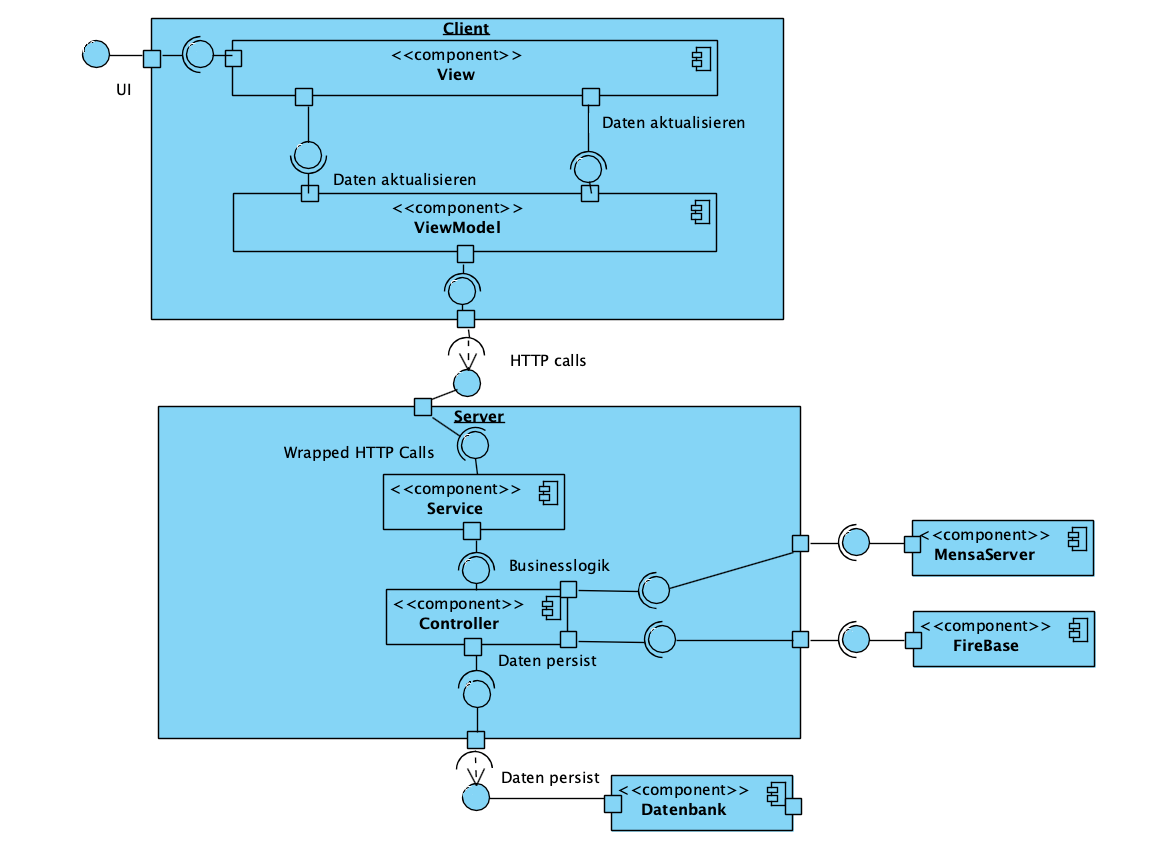
\includegraphics[width=1.1\textwidth]{Objektdiagramme/komponentDiagramm.png}
\section{Komponentenbeschreibung}
\subsection{Client}
Die Client Seite bedient sich der MVVM Architektur. Die View dient zum anzeigen von Daten, sie beinhaltet alle grafischen Elemente, stellt also die GUI dar. Im Model werden die Daten gehalten und Funktionen zur Manipulation der Daten bereitgestellt.
Das Viewmodel enthält die Darstellungslogik für die View und kapselt sie von der Anwendungslogik, die sich im Model befindet, ab.
View und Viewmodel sind durch Databinding nur lose gekoppelt, dadurch kann die View problemlos ausgetauscht werden bzw. können mehrere verscheidene Views (z.b. angepasst an Tablet, Desktop,...) zum selben Viewmodel existieren.
Das Datainding kann als bidirektionaler Beobachter verstanden werden: View und Viewmodel kennen die interne Struktur voneinander nicht, aber Benachrichtigen einander, wenn es Änderungen gibt. Diese lose Kopplung durch Databinding verbessert die Testbarkeit, da so View und Viewmodel unabhängig voneiander getestet werden können.

\subsection{Server}
Für die Server Seite wird die MVC Architektur verwendet.
Das Model ist für die Datenhaltung zuständig und beinhaltet/verwaltet eine Datenbank.  In unserem Fall wird die relationale Datenbank MySQL verwendet. Als Kommunikationsschnittstelle zwischen der Datenbank und den Controllern des Servers wird JPA (Java Persistance API) mit Hibernate genutzt.
View ist durch eine Schnittstelle gegeben, über die der Server Anfragen des Client empfängt und an den Controller delegiert. Der Controller führt diese Anfragen durch, indem er angefordere Daten aus dem Model holt oder neue Daten einfügt bzw Daten anpasst.

\subsection{Frameworks und Interfaces}
\subsection*{Hibernate und JPA}

Objektrelationales Mapping (ORM) ist eine Technik der Softwareentwicklung, mit der ein (in objektorientierten Programmiersprache geschriebenes) Programm seine Objekte in einer relationalen Datenbank ablegen kann. Dem Programm wird dazu eine objektorientierte Sicht auf die Tabellen und Beziehungen im Datenbankmangemantsystem (DBSM) geboten. \\  \\ Wir benutzen für ORM das Java Persistence Application Programming Interface (JPA). 
JPA ist eine API für Datenbankzugriffe und objektrelationales Mapping und muss durch einen sogenannten JPA Provider implemetiert werden. Wir verwenden hierzu das Framework Hibernate.\\ \\ Hibernate ermöglicht es normale Objekte (Plain Old Java Object, POJO) in relationalen Datenbanken zu speichern und aus den Datensätzen der Datenbank Objekte zu erzeugen. \\
Hibernate bietet Kompatibilität mit verschiedenen Datenbanken, sodass die von uns verwendete Datenbank MySQL leicht gegen eine andere relationale Datenbank ausgetauscht werden kann.

\subsection*{Spring Boot}

Spring Boot ist ein Framework, welches es erleichtern soll Java und Java EE Anwendungen zu schreiben und gute Programmierpraktiken zu fördern. Es ist eine vereinfachte Form des Spring Frameworks und bietet viele dessen Funktionalitäten auf schnell zu integierbarem Wege an. \\ \\
Wir benutzen Spring Boot, um schnell eine exportierbare direkt einsatzfähige Anwendung schreiben zu können und um Funktionalitäten wie Dependecy Injection nutzen zu können.

\subsection*{Firebase}
Firebase ist ein Framework, das viele Services bietet um die Entwicklung und die Handhabung der Infrastruktur von mobilen und Webanwendungen zu vereinfachen. Es übernimmt für uns die Registrierung, Speicherung und Organisation von Nutzerdaten, die wir für die Verwaltung von Accounts benötigen. \\ \\
Wir nutzen von den Services die Firebase bietet die Registrierung und Anmeldung mit einer Email-Adresse und einem Passwort, sowie die Möglichkeit zur Wiederherstellung des Passworts. Firebase bietet viele weitere Funktionalitäten, wie Push Notifications, an, die wir, bei Bedarf, in Zukunft nutzen können, um Wunschkriterien zu implementieren.
\chapter{Feinentwurf}
\section{Klassen des Clients}

%---------------------Javadocs für Client Model---------------%

\subsection{package.edu.kit.mensameet.client.model}
\begin{center}
	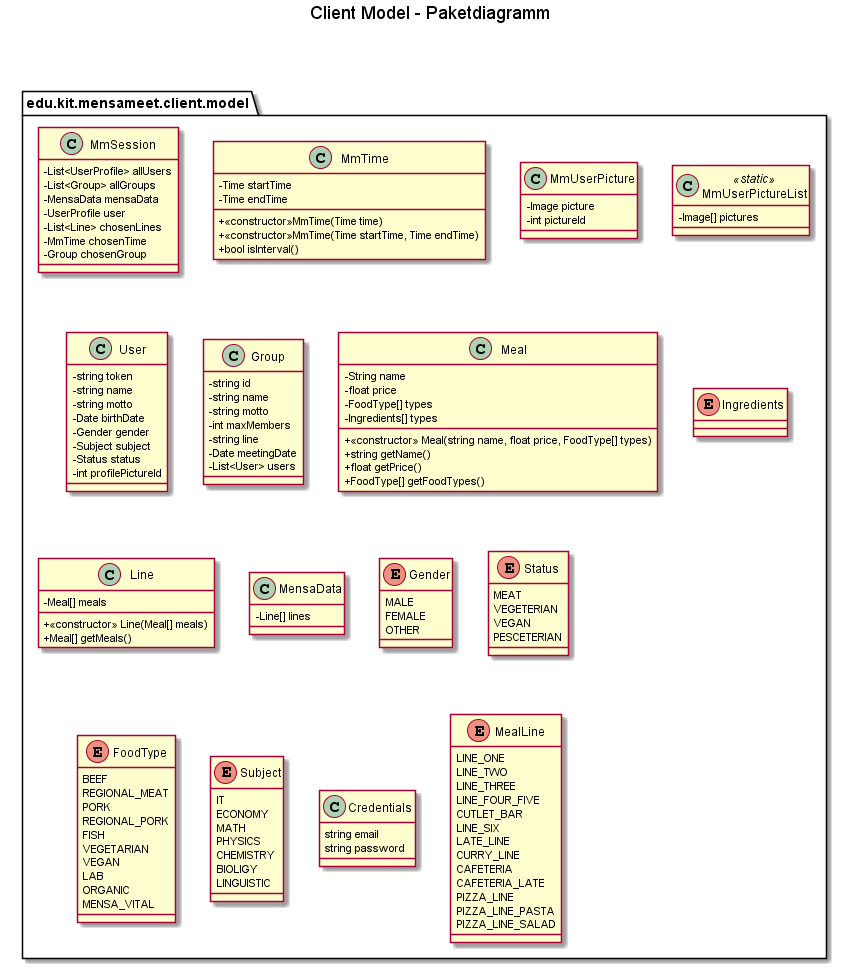
\includegraphics[width=0.93\textwidth]{GUI/frontend-package-model.png}
\end{center} 

%---------------

\subsubsection{Class MmSession}
\subsubsection*{Beschreibung}
In dieser Klasse können die Daten einer Sitzung wie Benutzer, ausgewählte Zeit, ausgewählte Linien und die ausgewählte Gruppe gespeichert werden. Bei ihrer Erzeugung werden zusätzlich noch Listen aller Benutzer bzw. Gruppen sowie die Mensadaten hineingeladen.

%---------------

\subsubsection{Class MmTime}
\subsubsection*{Beschreibung}
Diese Klasse kann eine Zeit oder einen Zeitraum speichern.

\subsubsection*{Konstruktoren}
\begin{addmargin}[25pt]{0pt}
\begin{itemize}

\item \texttt{MmTime(Time time)}\\
	Dieser Konstruktor legt eine Zeit an.

	\subsubsection*{Parameter}
	\begin{itemize}
	\item time \\
		Zeit.
	\end{itemize}

\item \texttt{MmTime(Time startTime, Time endTime)}\\
	Dieser Konstruktor legt einen Zeitraum an.

	\subsubsection*{Parameter}
	\begin{itemize}
	\item startTime \\
	Startzeit.
	\item endTime \\
	Endzeit.
	\end{itemize}

\end{itemize}
\end{addmargin}

\subsubsection*{Methoden}
\begin{addmargin}[25pt]{0pt}
\begin{itemize}

\item \texttt{bool isInterval()}\\
	Diese Methode gibt zurück, ob es sich um ein Zeitintervall handelt.

	\subsubsection*{Rückgabewert}
	Ob Zeitintervall.

\end{itemize}
\end{addmargin}

%---------------

\subsubsection{Class MmUserPicture}
\subsubsection*{Beschreibung}
Diese Klasse enthält eine Profilbilddatei mit zugehöriger Id.

%---------------

\subsubsection{Static class MmUserPictureList}
\subsubsection*{Beschreibung}
Diese Klasse enthält die Liste aller möglichen Profilbilder.


\subsubsection{Class Group}
Die folgenden Klassen enthalten Standardkonstruktoren, die nicht explizit aufgeführt werden: User, Group.
\subsubsection*{Beschreibung}
Dies ist eine Datenhalterklasse für eine Gruppe. 

\subsection{Class User}
\subsection*{Beschreibung}
Dies ist eine Datenhalterklasse für einen User.

\subsection{Class Credentials}
\subsection*{Beschreibung}
Diese Klasse beschreibt die Zugangsdaten (engl. Crendentials) eines Nutzers.

\subsection{Class MensaData}
\subsection*{Beschreibung}
Diese Klasse beinhaltet den Speiseplan der Mensa des aktuellen Tages.

\subsection{Class Line}
\subsection*{Beschreibung}
Diese Klasse beschreibt den Speiseplan der einzelnen Linien bzw. Werke an der Mensa.

\subsection{Class Meal}
\subsection*{Beschreibung}
Diese Klasse beschreibt die einzelnen Speisen die an der Mensa angeboten werden.
Dazu gehören die Zutaten (enum Ingredients) und der Typ (enum Foodtype).

\subsection{Class Preferences}
\subsection*{Beschreibung}
In dieser Klasse sind die Preferenzen des Nutzers zur Gruppensuche.

\subsubsection{Enum Gender}
\subsection*{Beschreibung}
Die Geschlechter, die zu einem User gehören können. \\
\textit{MALE} - das männliche Geschlecht \\
\textit{FEMALE} - das weibliche Geschlecht \\
\textit{OTHER} - weder männlicht, noch weiblich \\

\subsubsection{Enum Subject}
\subsection*{Beschreibung}
Die Fachrichtungen die ein User haben kann: \\ \\
\textit{Angewandte Geowissenschaften}\\
\textit{Architektur}\\
\textit{Bauingenieurwese}\\
\textit{Bioingenieurwesen}\\
\textit{Biologie}\\
\textit{Chemie}\\
\textit{Chemieingenieurwesen und Verfahrenstechnik}\\
\textit{Chemische Biologie}\\
\textit{Deutsch}\\
\textit{Elektro- und Informationstechnik}\\
\textit{Energy Engineering and Management}\\
\textit{Europäische Kultur und Ideengeschichte}\\
\textit{Financial Engineering}\\
\textit{Funktionaler und Konstruktiver Ingenieurbau-Engineering Structures}\\
\textit{Geodäsie und Geoinformatik}\\
\textit{Geographie}\\
\textit{Geoökologie}\\
\textit{Geophysik}\\
\textit{Germanistik}\\
\textit{Information Systems Engineering and Management} \\
\textit{Informatik}\\
\textit{Ingenieurpädagogik}\\
\textit{Kunstgeschichte}\\
\textit{Lebensmittelchemie}\\
\textit{Management of Product Development} \\
\textit{Maschinenbau}\\
\textit{Materialwissenschaft und Werkstofftechnik}\\
\textit{Mathematik}\\
\textit{Mechanical Engineering} \\
\textit{Mechatronik und Informationstechnik} \\
\textit{Meteorologie}\\
\textit{Mobilität und Infrastruktur}\\
\textit{Mobility Systems Engineering and Management}\\
\textit{Naturwissenschaft und Technik} \\
\textit{Optics and Photonics}\\
\textit{Pädagogik}\\
\textit{Philosophie/Ethik}\\
\textit{Physik}\\
\textit{Production and Operations Management}\\
\textit{Regionalwissenschaft}\\
\textit{Remote Sensing and Geoinformatics}\\
\textit{Sport}\\
\textit{Sportwissenschaft}\\
\textit{Technische Volkswirtschaftslehre} \\
\textit{Technomathematik}\\
\textit{Water Science and Engineering}\\
\textit{Wirtschaftsinformatik}\\
\textit{Wirtschaftsingenieurwesen}\\
\textit{Wirtschaftsmathematik}\\
\textit{Wissenschaft-Medien-Kommunikation}\\



\subsubsection{Enum Status}
\subsection*{Beschreibung}
Der Stauts den ein User haben kann: 
\\ \\ \textit{Professor} - Ein/e Professor/in oder Dozent/in \\
\textit{CollegeStudent} -  Ein/e Schüler-Student/in \\ 
\textit{Apprentice} - Ein/e Auszubildende/r \\
\textit{Student} - Ein/e reguläre/r Student/in \\
\textit{Other} - Sonstiges \\

\newpage
\subsubsection{Enum FoodType}
\subsection*{Beschreibung}
Die Sorten von Essen die es gibt und die man Gerichten zuordnen kann:
\\ \\ \textit{BEEF \\
 REGIONAL\_MEAT \\
 PORK \\
 REGIONAL\_PORK \\
 FISH \\
 VEGETARIAN \\
 VEGAN \\
 LAB \\
 ORGANIC \\
 MENSA\_VITAL \\
}

\subsubsection{Enum Ingredient}
\subsection*{Beschreibung}
Die Inhaltsstoffe, die in einem Gericht enthalten sein können: \\
\\
\textit{(1) mit Farbstoff \\
(2) mit Konservierungsstoff \\
(3) mit Antioxidationsmittel \\
(4) mit Geschmacksverstärker \\
(5) mit Phosphat \\
(6) Oberfläche gewachst \\
(7) geschwefelt \\
(8) Oliven geschwärzt \\
(9) mit Süßungsmittel \\
(10) kann bei übermäßigem Verzehr abführend wirken \\
(11) enthält eine Phenylalaninquelle \\
(12) kann Restalkohol enthalten \\
(14) aus Fleischstücken zusammengefügt \\
(15) mit kakaohaltiger Fettglasur \\
(27) aus Fischstücken zusammengefügt \\
(R) enthält Rindfleisch \\
(RAT) enthält regionales Rindfleisch aus artgerechter Tierhaltung \\
(S) enthält Schweinefleisch \\
(SAT) enthält regionales Schweinefleisch aus artgerechter Tierhaltung \\
(VEG) vegetarisches Gericht \\
(VG) veganes Gericht (ohne Fleischzusatz) \\
(B) kontrolliert biologischer Anbau / DE007 Öko Kontrollstelle \\
(MSC) MSC-zertifizierter Fisch \\
(MV) MensaVital \\
(LAB) mit tierischem Lab \\
(GER) mit Gelatine\\
(Gl) Glutenhaltiges Getreide \\
(We) Weizen \\
(Ro) Roggen \\
(Ge) Gerste \\
(Ha) Hafer \\
(Di) Dinkel \\
(Ka) Kamut \\
(Nu) Schalenfrüchte / Nüsse \\
(Ma) Mandeln \\
(Ha) Haselnüsse) \\ 
(Wa) Walnüsse \\
(Ca) Cashewnüsse \\
(Pe) Pekanüsse \\
(Pa) Paranüsse \\
(Pi) Pistazie \\
(Qu) Queenslandnüsse/Macadamianüsse \\
(Ei) Eier \\
(Er) Erdnüsse \\
(So) Soja \\
(Sn) Senf \\
(Kr) Krebstiere \\
(Fi) Fisch \\
(ML) Milch / Laktose \\
(Se) Sellerie \\
(Sf) Schwefeldioxid / Sulfit \\
(Sa) Sesam \\
(Lu) Lupine \\
(We) Weichtiere \\}
  

%------------ Java Doc for client view ---------------------

\newpage
\subsection{package.edu.kit.mensameet.client.view}

\begin{center}
	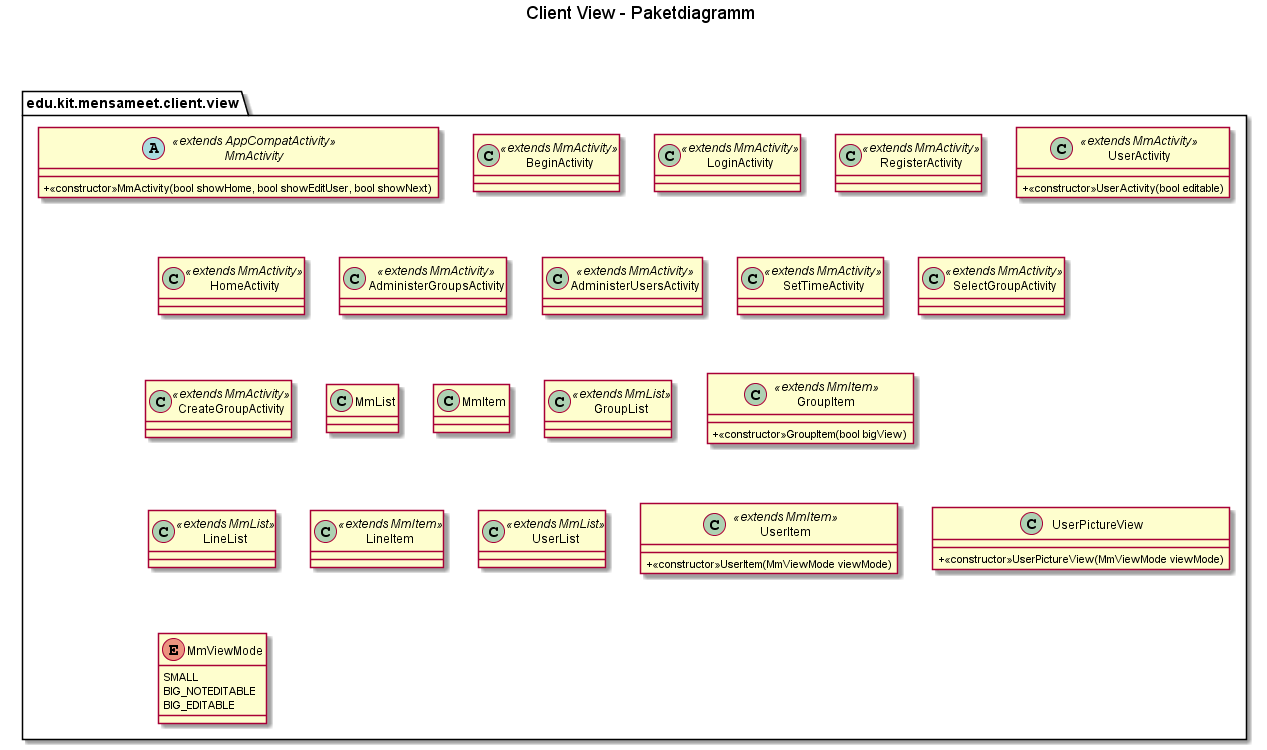
\includegraphics[width=1.1\textwidth]{GUI/frontend-package-view.png}
\end{center} 

\subsubsection{Abstract class MmActivity extends AppCompatActivity}
\subsubsection*{Beschreibung}
Diese abstrakte Klasse bildet das Grundgerüst für die Activitys.

\subsubsection*{Konstruktoren}
\begin{addmargin}[25pt]{0pt}
\begin{itemize}

\item \texttt{MmActivity(bool showHome, bool showEditUser, bool showNext)}\\
	
	Mit diesem Konstruktor lässt sich einstellen, welche Buttons angezeigt werden sollen.

	\subsubsection*{Parameter}
	\begin{itemize}
	\item showHome \\
		Zeige Home-Button an.
	\item showEditUser \\
		Zeige Profil-Button an.
	\item showNext \\
		Zeige Weiter-Button an.
	\end{itemize}

\end{itemize}
\end{addmargin}

%---------------------

\subsubsection{Class BeginActivity extends MmActivity}
\subsubsection*{Beschreibung}
Diese Oberfläche empfängt den Benutzer, wenn dieser die App das erste Mal startet. Er kann sich dann mit seinem bereits vorhandenem Account anmelden, falls er zum Beispiel nur ein neues Smartphone hat. Alternativ hat er die Möglichkeit sich zu registrieren und einen neuen Account anzulegen.

%---------------------

\subsubsection{Class LoginActivity extends MmActivity}
\subsubsection*{Beschreibung}
Diese Klasse bietet die Oberfläche der App, in der sich der Benutzer mit seinen Accountdaten anmelden kann.
%---------------------

\subsubsection{Class UserActivity extends MmActivity}
\subsubsection*{Beschreibung}
Diese Klasse zeigt ein Benutzerprofil auf einer ganzen Seite an.

\subsubsection*{Konstruktoren}
\begin{addmargin}[25pt]{0pt}
\begin{itemize}

\item \texttt{UserActivity(bool editable)}\\
	
	Mit diesem Konstruktor lässt sich einstellen, ob das Profil editierbar sein soll. 

	\subsubsection*{Parameter}
	\begin{itemize}
	\item editable \\
		Profil soll editierbar sein.
	\end{itemize}

\end{itemize}
\end{addmargin}

%---------------------

\subsubsection{Class HomeActivity extends MmActivity}
\subsubsection*{Beschreibung}
Diese Klasse bietet die Oberfläche der App, die als Homescreen für den Benutzer agiert. Der Benutzer kann hier seine bevorzugten Linien auswählen, an denen er gerne essen gehen würde.

%---------------------

\subsubsection{Class AdministerGroupsActivity extends MmActivity}
\subsubsection*{Beschreibung}
Diese Klasse zeigt für Administratoren eine Übersicht aller Gruppen an und stellt eine Löschtaste zur Verfügung. 

%---------------------

\subsubsection{Class AdministerUsersActivity extends MmActivity}
\subsubsection*{Beschreibung}
Diese Klasse zeigt für Administratoren eine Übersicht aller Benutzer an und stellt eine Löschtaste zur Verfügung.

%---------------------

\subsubsection{Class SelectGroupActivity extends MmActivity}
\subsubsection*{Beschreibung}
Diese Klasse bietet die Oberfläche der App, die dem Benutzer verschiedene Gruppen anzeigt, die anhand seiner davor eingegebenen Präferenzen ausgewählt wurden. Er kann hier die Gruppen antippen, um sich weitere Details über diese anzeigen zu lassen.

%---------------------

\subsubsection{Class CreateGroupActivity extends MmActivity}
\subsubsection*{Beschreibung}
Diese Klasse bietet die Oberfläche der App, die es dem Benutzer ermöglicht eine neue Gruppe zu gründen.

%---------------------

\subsubsection{Class MmList}
\subsubsection*{Beschreibung}
Diese Klasse dient als Grundgerüst für Listen in den Activitys. 

%---------------------

\subsubsection{Class MmItem}
\subsubsection*{Beschreibung}
Diese Klasse dient als Grundgerüst für Listenelemente in den Activitys. 

%---------------------

\subsubsection{Class GroupList extends MmList}
\subsubsection*{Beschreibung}
Diese Klasse bietet eine Oberfläche für eine Gruppenliste.

%---------------------

\subsubsection{Class GroupItem extends MmItem}
\subsubsection*{Beschreibung}
Diese Klasse bietet die Oberfläche der App, die dem Benutzer eine Gruppe und seine Teilnehmer anzeigt.
\subsubsection*{Konstruktoren}
\begin{addmargin}[25pt]{0pt}
\begin{itemize}

\item \texttt{GroupItem(bool bigView)}\\
	Mit diesem Konstruktor lässt sich einstellen, ob die Gruppenansicht in groß für eine Einzelseite oder, für Listen geeignet, in klein erfolgen soll. 

	\subsubsection*{Parameter}
	\begin{itemize}
	\item bigView \\
		Ob die Gruppenansicht groß sein soll. 
	\end{itemize}

\end{itemize}
\end{addmargin}

%---------------------

\subsubsection{Class LineList extends MmList}
\subsubsection*{Beschreibung}
Diese Klasse bietet eine Oberfläche für eine Liste von Mensalinien. 

%---------------------

\subsubsection{Class LineItem extends MmItem}
\subsubsection*{Beschreibung}
Diese Klasse bietet eine Oberfläche für ein Listenelement einer Mensalinien-Liste.

%---------------------

\subsubsection{Class UserList extends MmList}
\subsubsection*{Beschreibung}
Diese Klasse bietet eine Oberfläche für eine Benutzerliste.

%---------------------

\subsubsection{Class UserItem extends MmList}
\subsubsection*{Beschreibung}
Diese Klasse bietet die Oberfläche der App, die einen Benutzer anzeigt.
\subsubsection*{Konstruktoren}
\begin{addmargin}[25pt]{0pt}
\begin{itemize}

\item \texttt{UserItem(MmViewMode viewMode)}\\
	Mit diesem Konstruktor lässt sich einstellen, ob die Benutzeransicht in groß für eine Einzelseite, dabei bearbeitbar oder, für Listen geeignet, in klein erfolgen soll.


	\subsubsection*{Parameter}
	\begin{itemize}
	\item viewMode \\
		Anzeigeart: groß nur lesen, groß bearbeitbar oder klein.
	\end{itemize}

\end{itemize}
\end{addmargin}

%---------------------

\subsubsection{Class UserPictureView}
\subsubsection*{Beschreibung}
Diese Klasse kapselt die Darstellung eines Benutzerbildes.
\subsubsection*{Konstruktoren}
\begin{addmargin}[25pt]{0pt}
\begin{itemize}

\item \texttt{UserPictureView(MmViewMode viewMode)}\\
	Mit diesem Konstruktor lässt sich einstellen, ob das Benutzerbild in groß für eine Einzelseite, dabei bearbeitbar oder, für Listen geeignet, in klein erfolgen soll.

	\subsubsection*{Parameter}
	\begin{itemize}
	\item viewMode \\
		Anzeigeart: groß nur lesen, groß bearbeitbar oder klein.
	\end{itemize}

\end{itemize}
\end{addmargin}

%---------------------

\subsubsection{enum MmViewMode}
\subsubsection*{Beschreibung}
Anzeigearten
\textit{SMALL} - klein \\
\textit{BIGNOTEDITABLE} - gross und nicht bearbeitbar \\
\textit{BIGEDITABLE} - gross und bearbeitbar \\

%---------------------

\newpage
\subsection{package.edu.kit.mensameet.client.viewmodel}

%------------ Java Doc for client viewmodel ---------------------

\begin{center}
	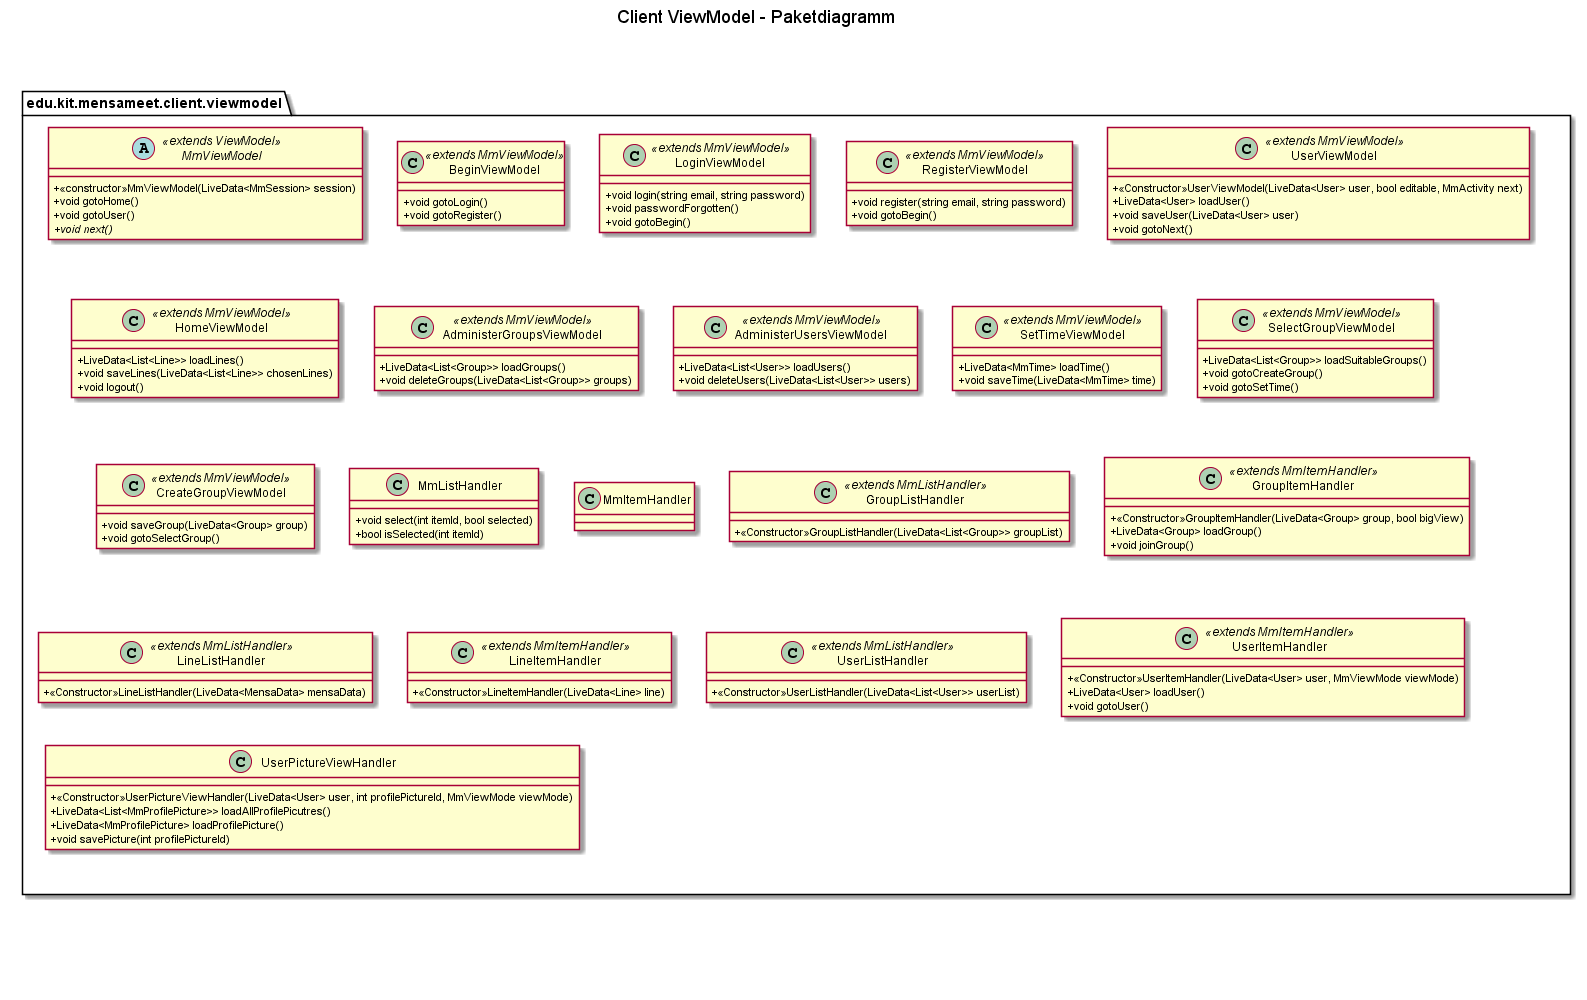
\includegraphics[width=1.1\textwidth]{GUI/frontend-package-viewmodel.png}
\end{center} 

\subsubsection{Abstract class MmViewModel extends ViewModel}
\subsubsection*{Beschreibung}
Diese abstrakte Klasse verwaltet alle Grundfunktionen, die die Klasse MmActivity ihren Unterklassen bereitstellt.


\subsubsection*{Konstruktoren}
\begin{addmargin}[25pt]{0pt}
\begin{itemize}

\item \texttt{MmViewModel(LiveData<MmSession> session)}\\
	
	Dieser Konstruktor nimmt ein MmSession-Element auf, in der die Daten der Sitzung gespeichert werden.

	\subsubsection*{Parameter}
	\begin{itemize}
	\item session \\
		Sitzungs-Klasse. Falls leer, wir eine neue erzeugt.
	\end{itemize}

\end{itemize}
\end{addmargin}

\subsubsection*{Methoden}
\begin{addmargin}[25pt]{0pt}
\begin{itemize}


\item \texttt{void gotoHome()}\\
	Diese Methode startet die Klasse HomeActivity.

\item \texttt{void gotoUser()}\\
	Diese Methode startet die Klasse UserActivity.
	
\item \texttt{abstract void next()}\\
	Diese Schablonenmethode kann von jeder abgeleiteten Klasse individuell für die folgende Activity angepasst werden.
	
\end{itemize}
\end{addmargin}

%---------------------

\subsubsection{Class BeginViewModel extends MmViewModel}
\subsubsection*{Beschreibung}
Diese Klasse verwaltet alle Funktionen, die die Klasse BeginActivity dem Benutzer bietet.

\subsubsection*{Methoden}
\begin{addmargin}[25pt]{0pt}
\begin{itemize}

\item \texttt{void gotoLogin()}\\
	Diese Methode startet die LoginActivity Klasse, damit der Benutzer sich mit seinem Account einloggen kann.

\item \texttt{void gotoRegister())}\\
	Diese Methode startet die RegisterActivity Klasse, damit der Benutzer sich mit seinen Daten registrieren und somit einen Account anlegen kann.

\end{itemize}
\end{addmargin}

%---------------

\subsubsection{Class LoginViewModel extends MmViewModel}
\subsubsection*{Beschreibung}
Diese Klasse verwaltet alle Funktionen, die die Klasse LoginActivity dem Benutzer bietet.

\subsubsection*{Methoden}
\begin{addmargin}[25pt]{0pt}
\begin{itemize}

\item \texttt{login(string email, string password)}\\
	Diese Methode leitet die Anmeldedaten an FireBase zur Überprüfung weiter und startet die Klasse HomeActivity, falls die Überprüfung erfolgreich war. Falls nicht wird eine Fehlermeldung in der LoginActivity erzeugt.
	\subsubsection*{Parameter}
	\begin{itemize}
	\item email \\
		FireBase-E-Mail-Adresse.
	\item password \\
		FireBase-Passwort.
	\end{itemize}

\item \texttt{passwordForgotten()}\\
	Diese Methode führt auf die FireBase-Seite bei Vergessen des Passworts.

\item \texttt{gotoBegin()}\\
	Diese Methode startet die Klasse BeginActivity wieder.

\end{itemize}
\end{addmargin}	


%---------------

\subsubsection{Class RegisterViewModel extends MmViewModel}
\subsubsection*{Beschreibung}
Diese Klasse verwaltet alle Funktionen, die die Klasse RegisterActivity dem Benutzer bietet.
\subsubsection*{Methoden}
\begin{addmargin}[25pt]{0pt}
\begin{itemize}

\item \texttt{register(string email, string password)}\\
	Diese Methode leitet Registrierungsdaten an FireBase zur Überprüfung weiter und erzeugt neue Profil, fallss diese erfolgreich war. Dann wird die Klasse UserActivity zur Profilvervollständigung gestartet. Falls nicht wird eine Fehlermeldung erzeugt.

	\subsubsection*{Parameter}
	\begin{itemize}
	\item email \\
		FireBase-E-Mail-Adresse.
	\item password \\
		FireBase-Passwort.
	\end{itemize}

\end{itemize}
\end{addmargin}	

%---------------

\subsubsection{UserViewModel extends MmViewModel}
\subsubsection*{Beschreibung}
Diese Klasse verwaltet alle Funktionen, die die Klasse UserActivity dem Benutzer bietet.

\subsubsection*{Konstruktoren}
\begin{addmargin}[25pt]{0pt}
\begin{itemize}

\item \texttt{UserViewModel(LiveData<User> user, bool editable, MmActivity next)}\\
Mit diesem Konstruktor lässt sich anzeigen, ob das Profil eine Bearbeitungsansicht sein soll. Außerdem lässt sich einstellen, welche Folgeseite aufgerufen wird.

	\subsubsection*{Parameter}
	\begin{itemize}
	\item LiveData<User> user \\
		Der bearbeitete Benutzer.
	\item bool editable \\
		Ob Bearbeitungsansicht aktiviert ist.
	\item MmActivity next \\
		Folgeseite.
	\end{itemize}

\end{itemize}
\end{addmargin}

\subsubsection*{Methoden}
\begin{addmargin}[25pt]{0pt}
\begin{itemize}


\item \texttt{LiveData<User> loadUser()}\\
	Diese Methode gibt den Benutzer zurück.

	\subsubsection*{Rückgabewert}
	Benutzer.

\item \texttt{void saveUser(LiveData<User> user)}\\
	Diese Methode speichert die Benutzerdaten.

	\subsubsection*{Parameter}
	\begin{itemize}
	\item user \\
		Benutzer.
	\end{itemize}
	
\item \texttt{void gotoNext()}\\
	Diese Methode startet die Folgeseite.
	
\end{itemize}
\end{addmargin}

%---------------

\subsubsection{Class HomeViewModel extends MmViewModel}
\subsubsection*{Beschreibung}
Diese Klasse verwaltet alle Funktionen, die die Klasse HomeActivity dem Benutzer bietet.

\subsubsection*{Methoden}
\begin{addmargin}[25pt]{0pt}
\begin{itemize}

\item \texttt{LiveData<List<Line> > loadLines()}\\
	Diese Methode lädt eine Liste mit dem Essensangebot der Mensalinien. 

	\subsubsection*{Rückgabewert}
	Liste des Essensangebots der Mensalinien.

\item \texttt{void saveLines(LiveData<List<Line> > chosenLines)}\\
	Diese Methode speichert die Linien, die der Benutzer als Favoriten angegeben hat und startet die Klasse SetTimeActivity.
	\subsubsection*{Parameter}
	\begin{itemize}
	\item chosenLines \\
	Liste der als Favoriten angegebenen Linien.
	\end{itemize}

\item \texttt{+void logout()}\\
    Diese Methode startet Klasse BeginActivity, wobei die MmSession-Klasse mit einer neuen ersetzt wird.

\end{itemize}
\end{addmargin}

%---------------

\subsubsection{Class AdministerGroupsViewModel extends MmViewModel}
\subsubsection*{Beschreibung}
Diese Klasse verwaltet alle Funktionen, die die Klasse AdministerGroupsActivity dem Benutzer bietet.

\subsubsection*{Methoden}
\begin{addmargin}[25pt]{0pt}
\begin{itemize}

\item \texttt{LiveData<List<Group> > loadGroups()}\\
	Diese Methode lädt eine Liste aller Gruppen.

	\subsubsection*{Rückgabewert}
	Liste aller Gruppen.

\item \texttt{deleteGroups(LiveData<List<Group> > groups)}\\
	Diese Methode löscht eine Menge von Gruppen.
	\subsubsection*{Parameter}
	\begin{itemize}
	\item groups \\
		Zu löschende Menge von Gruppen.
	\end{itemize}

\end{itemize}
\end{addmargin}

%---------------

\subsubsection{Class AdministerUsersViewModel extends MmViewModel}
\subsubsection*{Beschreibung}
Diese Klasse verwaltet alle Funktionen, die die Klasse AdministerUsersActivity dem Benutzer bietet.

\subsubsection*{Methoden}
\begin{addmargin}[25pt]{0pt}
\begin{itemize}

\item \texttt{LiveData<List<User> > loadUsers()}\\
	Diese Methode lädt eine Liste aller Benutzer.

	\subsubsection*{Rückgabewert}
	Liste aller Benutzer.

\item \texttt{void deleteUsers(LiveData<List<User> > users)}\\
Diese Methode löscht eine Menge von Benutzern.
	\subsubsection*{Parameter}
	\begin{itemize}
	\item users \\
		Zu löschende Menge von Benutzern.
	\end{itemize}

\end{itemize}
\end{addmargin}

%---------------

\subsubsection{Class SetTimeViewModel extends MmViewModel}
\subsubsection*{Beschreibung}
Diese Klasse verwaltet alle Funktionen, die die Klasse SetTimeActivity dem Benutzer bietet.

\subsubsection*{Methoden}
\begin{addmargin}[25pt]{0pt}
\begin{itemize}

\item \texttt{LiveData<MmTime> loadTime()}\\
	Diese Methode lädt die bereits eingestellte Zeit/Zeitraum.

	\subsubsection*{Rückgabewert}
	Bereits eingestellte Zeit/Zeitraum.

\item \texttt{void saveTime(LiveData<MmTime> time)}\\
Diese Methode speichert die eingegebene Zeit/Zeitraum zur weiteren Verwendung für die nachfolgenden Funktionen in der App ab.

	\subsubsection*{Parameter}
	\begin{itemize}
	\item time \\
		Zu speichernde Zeit/Zeitraum
	\end{itemize}

\end{itemize}
\end{addmargin}

%---------------

\subsubsection{Class SelectGroupViewModel extends MmViewModel}
\subsubsection*{Beschreibung}
Diese Klasse verwaltet alle Funktionen, die die Klasse SelectGroupActivity dem Benutzer bietet.

\subsubsection*{Methoden}
\begin{addmargin}[25pt]{0pt}
\begin{itemize}

\item \texttt{LiveData<List<Group> > loadSuitableGroups()}\\
	Diese Methode lädt alle Gruppen, die zu den gespeicherten Kriterien in der MmSession-Klasse passen.

	\subsubsection*{Rückgabewert}
	Alle passenden Gruppen.

\item \texttt{void gotoCreateGroup()}\\
Diese Methode startet die Klasse CreateNewGroupActivity.

\item \texttt{void gotoSetTime()}\\	
Diese Methode startet die Klasse SetTimeActivity.

\end{itemize}
\end{addmargin}

%---------------

\subsubsection{Class CreateGroupViewModel extends MmViewModel}
\subsubsection*{Beschreibung}
Diese Klasse verwaltet alle Funktionen, die die Klasse CreateGroupActivity dem Benutzer bietet.

\subsubsection*{Methoden}
\begin{addmargin}[25pt]{0pt}
\begin{itemize}

\item \texttt{void saveGroup(LiveData<Group> group)}\\
	Diese Methode speichert die Daten der neu angelegten Gruppe.

	\subsubsection*{Parameter}
	\begin{itemize}
	\item group \\
		Neue Gruppenklasse.
	\end{itemize}

\item \texttt{void gotoSelectGroup()}\\
Diese Methode startet die Klasse SelectGroupActivity.

\end{itemize}
\end{addmargin}

%---------------

\subsubsection{Class MmListHandler}
\subsubsection*{Beschreibung}
Diese Klasse verwaltet alle Funktionen, die die Klasse MmList dem Benutzer bietet.

\subsubsection*{Methoden}
\begin{addmargin}[25pt]{0pt}
\begin{itemize}

\item \texttt{void select(int itemId, bool selected)}\\
	Diese Methode setzt ein Element in der Liste auf (nicht) ausgewählt.

	\subsubsection*{Parameter}
	\begin{itemize}
	\item itemId \\
		Id des Elements der Liste.
	\item selected \\
		Ob das Element ausgewählt sein soll.
	\end{itemize}

\item \texttt{bool isSelected(int itemId)}\\
 Diese Methode gibt zurück, ob ein Element der Liste ausgewählt ist.  
	\subsubsection*{Parameter}
	\begin{itemize}
	\item itemId \\
		Id des Elements der Liste
	\end{itemize}

'   \subsubsection*{Rückgabewert}
	Ob das Element ausgewählt ist.

\end{itemize}
\end{addmargin}

%---------------

\subsubsection{Class MmItemHandler}
\subsubsection*{Beschreibung}
Diese Klasse verwaltet alle Funktionen, die die Klasse MmItem dem Benutzer bietet.

%---------------

\subsubsection{Class GroupListHandler extends MmListHandler}
\subsubsection*{Beschreibung}
Diese Klasse verwaltet alle Funktionen, die die Klasse GroupList dem Benutzer bietet.

\subsubsection*{Konstruktoren}
\begin{addmargin}[25pt]{0pt}
\begin{itemize}

\item \texttt{GroupListHandler(LiveData<List<Group> > groupList)}\\
	Dieser Konstruktor erzeugt aus einer Gruppenliste die Klasse.

	\subsubsection*{Parameter}
	\begin{itemize}
	\item groupList \\
		Gruppenliste.
	\end{itemize}

\end{itemize}
\end{addmargin}

%---------------

\subsubsection{Class GroupItemHandler extends MmItemHandler}
\subsubsection*{Beschreibung}
Diese Klasse verwaltet alle Funktionen, die die Klasse GroupItem dem Benutzer bietet.

\subsubsection*{Konstruktoren}
\begin{addmargin}[25pt]{0pt}
\begin{itemize}

\item \texttt{GroupItemHandler(LiveData<Group> group, bool bigView)}\\
	Dieser Konstruktor erzeugt aus einer Gruppe die Klasse und gibt dabei an, ob die Anzeige im zugehörigen GroupItem groß oder klein ist, was Unterschiede in der Funktionalität zur Folge haben können soll. 

	\subsubsection*{Parameter}
	\begin{itemize}
	\item group \\
		Gruppe.
	\item bigView \\
		Ob die Anzeige im zugehörigen GroupItem groß ist. 
	\end{itemize}

\end{itemize}
\end{addmargin}

\subsubsection*{Methoden}
\begin{addmargin}[25pt]{0pt}
\begin{itemize}

\item \texttt{LiveData<Group> loadGroup}\\
	Lädt die gespeicherte Gruppe.

	\subsubsection*{Rückgabewert}
	Gespeicherte Gruppe.

\item \texttt{void joinGroup()}\\
	Diese Methode fügt den Benutzer in die Gruppe hinzu.

\end{itemize}
\end{addmargin}

%---------------

\subsubsection{Class LineListHandler extends MmListHandler}
\subsubsection*{Beschreibung}
Diese Klasse verwaltet alle Funktionen, die die Klasse LineList dem Benutzer bietet.

\subsubsection*{Konstruktoren}
\begin{addmargin}[25pt]{0pt}
\begin{itemize}

\item \texttt{LineListHandler(LiveData<MensaData> mensaData)}\\
	Dieser Konstruktor erzeugt aus den Mensadaten die Klasse.

	\subsubsection*{Parameter}
	\begin{itemize}
	\item mensaData \\
		Mensadaten.
	\end{itemize}

\end{itemize}
\end{addmargin}

%---------------

\subsubsection{Class LineItemHandler extends MmItemHandler}
\subsubsection*{Beschreibung}
Diese Klasse verwaltet alle Funktionen, die die Klasse LineItem dem Benutzer bietet.

\subsubsection*{Konstruktoren}
\begin{addmargin}[25pt]{0pt}
\begin{itemize}

\item \texttt{LineItemHandler(LiveData<Line> line)}\\
	Dieser Konstruktor erzeugt aus den Daten einer Mensalinie die Klasse.

	\subsubsection*{Parameter}
	\begin{itemize}
	\item line \\
		Daten einer Mensalinie.
	\end{itemize}

\end{itemize}
\end{addmargin}

%---------------

\subsubsection{Class UserListHandler extends MmListHandler}
\subsubsection*{Beschreibung}
Diese Klasse verwaltet alle Funktionen, die die Klasse UserList dem Benutzer bietet.

\subsubsection*{Konstruktoren}
\begin{addmargin}[25pt]{0pt}
\begin{itemize}

\item \texttt{UserListHandler(LiveData<List<User> > userList)}\\
	Dieser Konstruktor erzeugt aus einer Benutzerliste die Klasse.

	\subsubsection*{Parameter}
	\begin{itemize}
	\item userList \\
		Benutzerliste.
	\end{itemize}

\end{itemize}
\end{addmargin}

%---------------

\subsubsection{Class UserItemHandler extends MmItemHandler}
\subsubsection*{Beschreibung}
Diese Klasse verwaltet alle Funktionen, die die Klasse UserItem dem Benutzer bietet.

\subsubsection*{Konstruktoren}
\begin{addmargin}[25pt]{0pt}
\begin{itemize}

\item \texttt{UserItemHandler(LiveData<User> user, MmViewMode viewMode)}\\
	Dieser Konstruktor erzeugt aus einem Benutzer und dem Anzeigemodus (groß nur lesen, groß bearbeitbar oder klein) die Klasse. Der Anzeigemodus soll Änderungen in der Funktionalität zur Folge haben können.

	\subsubsection*{Parameter}
	\begin{itemize}
	\item user \\
		Benutzer.
	\item viewMode \\
		Anzeigemodus (groß nur lesen, groß bearbeitbar oder klein).
	\end{itemize}

\end{itemize}
\end{addmargin}

\subsubsection*{Methoden}
\begin{addmargin}[25pt]{0pt}
\begin{itemize}

\item \texttt{LiveData<User> loadUser()}\\
	Lädt den gespeicherten Benutzer.

  \subsubsection*{Rückgabewert}
	Gespeicherter Benutzer.

\end{itemize}
\end{addmargin}

%---------------

\subsubsection{Class UserPictureViewHandler}
\subsubsection*{Beschreibung}
Diese Klasse verwaltet alle Funktionen, die die Klasse UserPictureView dem Benutzer bietet.

\subsubsection*{Konstruktoren}
\begin{addmargin}[25pt]{0pt}
\begin{itemize}

\item \texttt{UserPictureViewHandler(LiveData<User> user, int profilePictureId, MmViewMode viewMode)}\\
	Dieser Konstruktor erzeugt die Klasse aus dem zum Bild gehörigen Benutzer, der Id des Bildes und dem Anzeigemodus (groß nur lesen, groß bearbeitbar oder klein). Der Anzeigemodus soll Änderungen in der Funktionalität zur Folge haben können.

	\subsubsection*{Parameter}
	\begin{itemize}
	\item user \\
	Benutzer.
	\item profilePictureId \\
	Id des Bildes.
	\item viewMode \\
	Anzeigemodus (groß nur lesen, groß bearbeitbar oder klein).
	\end{itemize}

\end{itemize}
\end{addmargin}

\subsubsection*{Methoden}
\begin{addmargin}[25pt]{0pt}
\begin{itemize}

\item \texttt{LiveData<List<MmProfilePicture> > loadAllProfilePicutres()}\\
	Lädt eine Liste aller möglichen Profilbilder, damit der Benutzer in der Klasse UserPictureView eins auswählen kann.

  \subsubsection*{Rückgabewert}
	Liste aller möglichen Profilbilder.

\item \texttt{LiveData<MmProfilePicture> loadProfilePicture()}\\
	Lädt das gespeicherte Profilbild.

  \subsubsection*{Rückgabewert}
	Das gespeicherte Profilbild.

\item \texttt{void savePicture(int profilePictureId)}\\
Speichert ein ausgewähltes Profilbild.
	\subsubsection*{Parameter}
	\begin{itemize}
	\item profilePictureId \\
	Id des ausgewählten Bildes.
	\end{itemize}

\end{itemize}
\end{addmargin}

\newpage
\subsection{Ausgewählte Klassenbeziehungen des Clients}
\begin{center}
	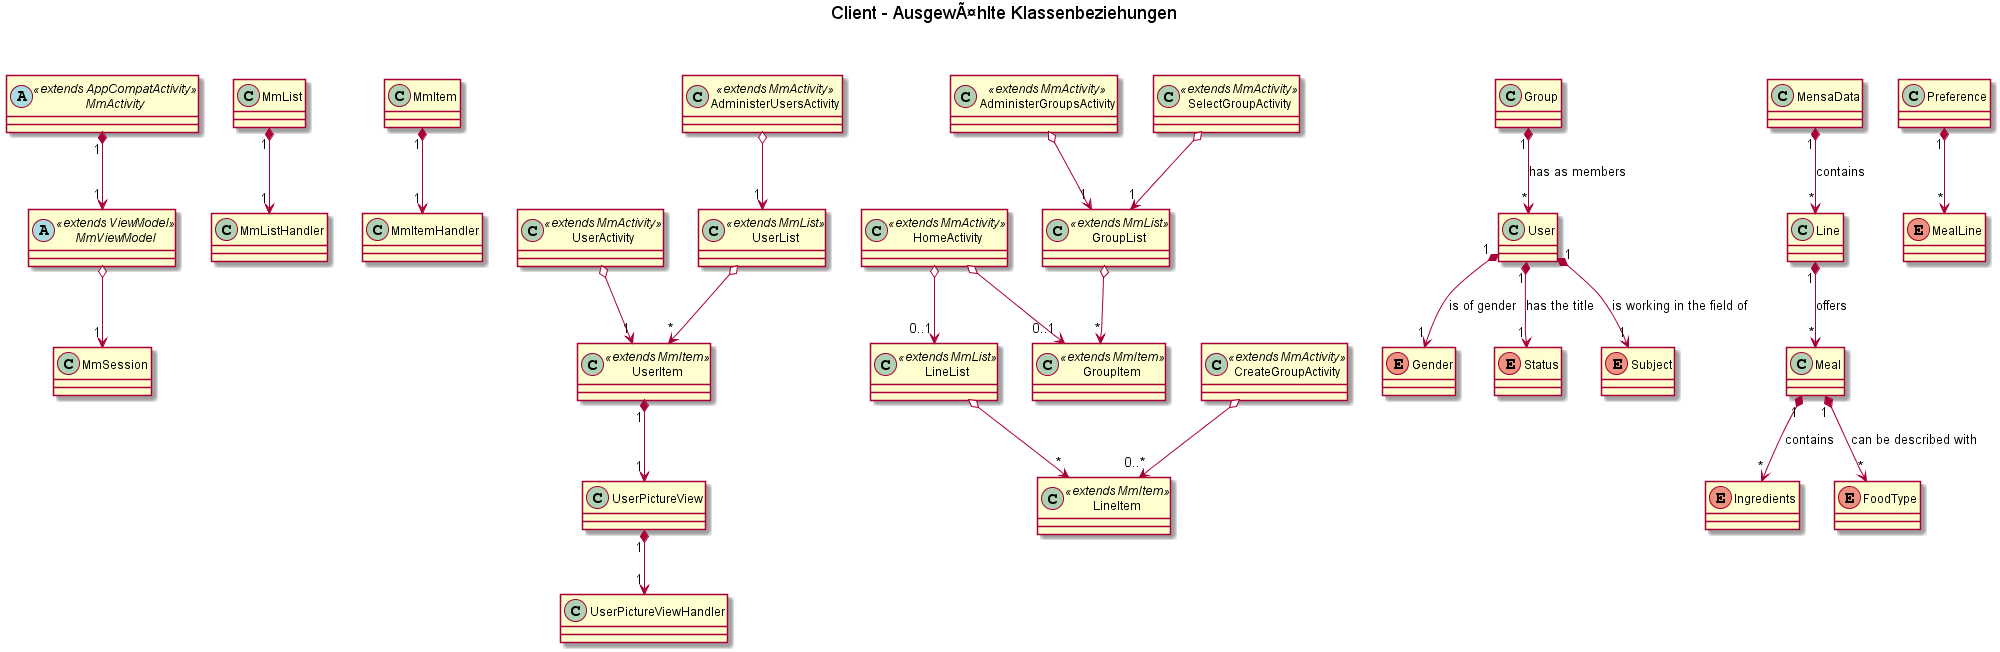
\includegraphics[width=1.1\textwidth]{GUI/frontend_beziehungen.png}
\end{center} 


%Klassen des Servers%
\section{Klassen des Server}

\subsection{Klassendiagramm}
	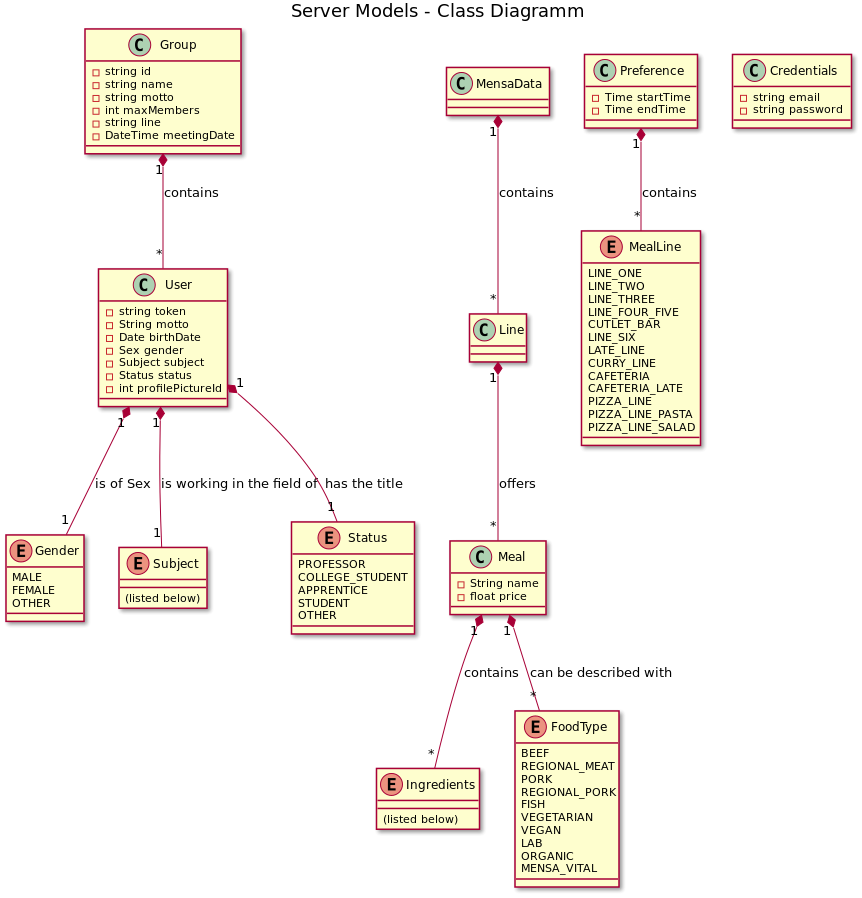
\includegraphics[width=1\textwidth]{Klassendiagramme/serverModelsCD.png}
\newpage
\subsection{package.edu.kit.mensameet.server.model}
%Javadocs für Model%
\subsubsection{Class Group}
Die folgenden Klassen enthalten Standardkonstruktoren, die nicht explizit aufgeführt werden: User, Group.
\subsubsection*{Beschreibung}
Dies ist eine Datenhalterklasse für eine Gruppe. 

\subsubsection{Class User}
\subsection*{Beschreibung}
Dies ist eine Datenhalterklasse für einen User.

\subsubsection{Class Crendentials}
\subsection*{Beschreibung}
Diese Klasse beschreibt die Zugangsdaten (engl. Crendentials) eines Nutzers.

\subsubsection{Class MensaData}
\subsection*{Beschreibung}
Diese Klasse beinhaltet den Speiseplan der Mensa des aktuellen Tages.

\subsubsection{Class Line}
\subsection*{Beschreibung}
Diese Klasse beschreibt den Speiseplan der einzelnen Linien bzw. Werke an der Mensa.

\subsubsection{Class Meal}
\subsection*{Beschreibung}
Diese Klasse beschreibt die einzelnen Speisen die an der Mensa angeboten werden.
Dazu gehören die Zutaten (enum Ingredients) und der Typ (enum Foodtype).

\subsubsection{Class Preferences}
\subsection*{Beschreibung}
In dieser Klasse sind die Preferenzen des Nutzers zur Gruppensuche.


\subsubsection{Enum Gender}
\subsection*{Beschreibung}
Die Geschlechter, die zu einem User gehören können. \\
\textit{MALE} - das männliche Geschlecht \\
\textit{FEMALE} - das weibliche Geschlecht \\
\textit{OTHER} - weder männlicht, noch weiblich \\

\subsubsection{Enum Subject}
\subsection*{Beschreibung}
Die Fachrichtungen die ein User haben kann: \\ \\
\textit{Angewandte Geowissenschaften}\\
\textit{Architektur}\\
\textit{Bauingenieurwese}\\
\textit{Bioingenieurwesen}\\
\textit{Biologie}\\
\textit{Chemie}\\
\textit{Chemieingenieurwesen und Verfahrenstechnik}\\
\textit{Chemische Biologie}\\
\textit{Deutsch}\\
\textit{Elektro- und Informationstechnik}\\
\textit{Energy Engineering and Management}\\
\textit{Europäische Kultur und Ideengeschichte}\\
\textit{Financial Engineering}\\
\textit{Funktionaler und Konstruktiver Ingenieurbau-Engineering Structures}\\
\textit{Geodäsie und Geoinformatik}\\
\textit{Geographie}\\
\textit{Geoökologie}\\
\textit{Geophysik}\\
\textit{Germanistik}\\
\textit{Information Systems Engineering and Management} \\
\textit{Informatik}\\
\textit{Ingenieurpädagogik}\\
\textit{Kunstgeschichte}\\
\textit{Lebensmittelchemie}\\
\textit{Management of Product Development} \\
\textit{Maschinenbau}\\
\textit{Materialwissenschaft und Werkstofftechnik}\\
\textit{Mathematik}\\
\textit{Mechanical Engineering} \\
\textit{Mechatronik und Informationstechnik} \\
\textit{Meteorologie}\\
\textit{Mobilität und Infrastruktur}\\
\textit{Mobility Systems Engineering and Management}\\
\textit{Naturwissenschaft und Technik} \\
\textit{Optics and Photonics}\\
\textit{Pädagogik}\\
\textit{Philosophie/Ethik}\\
\textit{Physik}\\
\textit{Production and Operations Management}\\
\textit{Regionalwissenschaft}\\
\textit{Remote Sensing and Geoinformatics}\\
\textit{Sport}\\
\textit{Sportwissenschaft}\\
\textit{Technische Volkswirtschaftslehre} \\
\textit{Technomathematik}\\
\textit{Water Science and Engineering}\\
\textit{Wirtschaftsinformatik}\\
\textit{Wirtschaftsingenieurwesen}\\
\textit{Wirtschaftsmathematik}\\
\textit{Wissenschaft-Medien-Kommunikation}\\



\subsubsection{Enum Status}
\subsection*{Beschreibung}
Der Stauts den ein User haben kann: 
\\ \\ \textit{Professor} - Ein/e Professor/in oder Dozent/in \\
\textit{CollegeStudent} -  Ein/e Schüler-Student/in \\ 
\textit{Apprentice} - Ein/e Auszubildende/r \\
\textit{Student} - Ein/e reguläre/r Student/in \\
\textit{Other} - Sonstiges \\

\newpage
\subsubsection{Enum FoodType}
\subsection*{Beschreibung}
Die Sorten von Essen die es gibt und die man Gerichten zuordnen kann:
\\ \\ \textit{BEEF \\
 REGIONAL\_MEAT \\
 PORK \\
 REGIONAL\_PORK \\
 FISH \\
 VEGETARIAN \\
 VEGAN \\
 LAB \\
 ORGANIC \\
 MENSA\_VITAL \\
}

\subsubsection{Enum Ingredient}
\subsection*{Beschreibung}
Die Inhaltsstoffe, die in einem Gericht enthalten sein können: \\
\\
\textit{(1) mit Farbstoff \\
(2) mit Konservierungsstoff \\
(3) mit Antioxidationsmittel \\
(4) mit Geschmacksverstärker \\
(5) mit Phosphat \\
(6) Oberfläche gewachst \\
(7) geschwefelt \\
(8) Oliven geschwärzt \\
(9) mit Süßungsmittel \\
(10) kann bei übermäßigem Verzehr abführend wirken \\
(11) enthält eine Phenylalaninquelle \\
(12) kann Restalkohol enthalten \\
(14) aus Fleischstücken zusammengefügt \\
(15) mit kakaohaltiger Fettglasur \\
(27) aus Fischstücken zusammengefügt \\
(R) enthält Rindfleisch \\
(RAT) enthält regionales Rindfleisch aus artgerechter Tierhaltung \\
(S) enthält Schweinefleisch \\
(SAT) enthält regionales Schweinefleisch aus artgerechter Tierhaltung \\
(VEG) vegetarisches Gericht \\
(VG) veganes Gericht (ohne Fleischzusatz) \\
(B) kontrolliert biologischer Anbau / DE007 Öko Kontrollstelle \\
(MSC) MSC-zertifizierter Fisch \\
(MV) MensaVital \\
(LAB) mit tierischem Lab \\
(GER) mit Gelatine\\
(Gl) Glutenhaltiges Getreide \\
(We) Weizen \\
(Ro) Roggen \\
(Ge) Gerste \\
(Ha) Hafer \\
(Di) Dinkel \\
(Ka) Kamut \\
(Nu) Schalenfrüchte / Nüsse \\
(Ma) Mandeln \\
(Ha) Haselnüsse) \\ 
(Wa) Walnüsse \\
(Ca) Cashewnüsse \\
(Pe) Pekanüsse \\
(Pa) Paranüsse \\
(Pi) Pistazie \\
(Qu) Queenslandnüsse/Macadamianüsse \\
(Ei) Eier \\
(Er) Erdnüsse \\
(So) Soja \\
(Sn) Senf \\
(Kr) Krebstiere \\
(Fi) Fisch \\
(ML) Milch / Laktose \\
(Se) Sellerie \\
(Sf) Schwefeldioxid / Sulfit \\
(Sa) Sesam \\
(Lu) Lupine \\
(We) Weichtiere \\}


%------------ Java Doc for the sever view package ---------------------

\newpage
\subsection{package.edu.kit.mensameet.server.view}

\begin{center}
	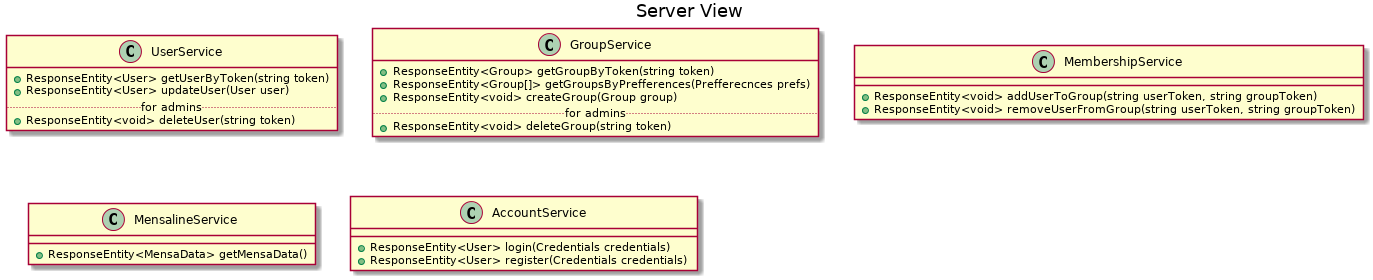
\includegraphics[width=1.1\textwidth]{Klassendiagramme/serverViewCD.png}
\end{center} 
Alle folgenden Klassen haben keine Konstruktoren, da sie keine Instanzen besitzen sollen,sondern lediglich statische Funktionen beinhalten, die die Schnittstelle des Servers bilden. Da alle Rückgabetypen vom Typ ResponseEntity sind werden auch alle http status codes die auftreten können beschrieben.

\subsubsection{Class UserService}
\subsubsection*{Beschreibung}
Diese Klasse stellt die für den Client benötigten Funktionen bereit um User Daten abzufragen und zu bearbeiten. 

\subsubsection*{Methoden}
\begin{addmargin}[25pt]{0pt}
\begin{itemize}

\item \texttt{ResponseEntity<User> getUserByToken(string token)}\\
	Liefert den User mit dem übergebenen Token. 

	\subsubsection*{Parameter}
	\begin{itemize}
	\item token \\
		Der Token, mit dem der User eindeutig identifizierbar ist.
	\end{itemize}

	\subsubsection*{Rückgabewert}
	Der gesuchte User als ResponseEntity mit status code 200.
	Status code 404, falls der User mit dem Token nicht existiert.

\item \texttt{ResponseEntity<User> updateUser(User user)}\\
	Updated den User auf dem Server mit dem übereinstimmenden Token.

	\subsubsection*{Parameter}
	\begin{itemize}
	\item user \\
		Der User der geupdated werden soll.
	\end{itemize}

	\subsubsection*{Rückgabewert}
	Der geupdatete User als ResponseEntity mit status code 200.
	Status code 404, falls der User mit dem Token nicht existiert.
	
\item \texttt{ResponseEntity<void> deleteUser(string token)}\\
	Löscht den User auf dem Server mit dem übereinstimmenden Token.

	\subsubsection*{Parameter}
	\begin{itemize}
	\item token \\
		Der Token des User, der gelöscht werden soll.
	\end{itemize}

	\subsubsection*{Rückgabewert}
	Status code 200, falls der User gefunden und gelöscht werden konnte.
	Status code 404, falls der User mit dem Token nicht existiert.
	
\end{itemize}
\end{addmargin}

%---------------------

\subsubsection{Class GroupService}
\subsubsection*{Beschreibung}
Diese Klasse stellt die für den Client benötigten Funktionen bereit um Gruppen Daten abzufragen und zu bearbeiten. 

\subsubsection*{Methoden}
\begin{addmargin}[25pt]{0pt}
\begin{itemize}

\item \texttt{ResponseEntity<Group> getGroupByToken(string token)}\\
	Liefert die Gruppe mit dem übergebenen Token. 

	\subsubsection*{Parameter}
	\begin{itemize}
	\item token \\
		Der Token, mit dem die Gruppe eindeutig identifizierbar ist.
	\end{itemize}

	\subsubsection*{Rückgabewert}
	Die gesuchte Gruppe als ResponseEntity mit status code 200.
	Status code 404, falls die Gruppe mit dem Token nicht existiert.

\item \texttt{ResponseEntity<Group[]> getGroupsByPrefferences(Prefferecnces prefs)}\\
	Liefert alle Gruppen, die zu den übergebenen Präferenzen passen.

	\subsubsection*{Parameter}
	\begin{itemize}
	\item prefs \\
		Die Präferenzen, mit denen die Gruppen gesucht werden sollen.
	\end{itemize}

	\subsubsection*{Rückgabewert}
	Ein Array aller passenden Gruppen als ResponseEntity mit status code 200.
	
\item \texttt{ResponseEntity<void> createGroup(Group group)}\\
	Erstellt eine Gruppe auf dem Server.

	\subsubsection*{Parameter}
	\begin{itemize}
	\item group \\
		Die Gruppe, die erstellt werden soll.
	\end{itemize}

	\subsubsection*{Rückgabewert}
	Die erstellte Gruppe mit einen generierten token als ResponseEntity, mit status code 200.
	
\item \texttt{ResponseEntity<void> deleteGroup(string token)}\\
	Löscht die Gruppe auf dem Server mit dem übereinstimmenden Token.

	\subsubsection*{Parameter}
	\begin{itemize}
	\item token \\
		Der Token der Gruppe, die gelöscht werden soll.
	\end{itemize}

	\subsubsection*{Rückgabewert}
	Status code 200, falls die Gruppe gefunden und gelöscht werden konnte.
	Status code 404, falls die Gruppe mit dem Token nicht existiert.


\end{itemize}
\end{addmargin}

%---------------

\subsubsection{Class MembershipService}
\subsubsection*{Beschreibung}
Diese Klasse stellt die für den Client benötigten Funktionen bereit um die Mitgliedschaft von Usern bei Gruppen zu bearbeiten. 

\subsubsection*{Methoden}
\begin{addmargin}[25pt]{0pt}
\begin{itemize}

\item \texttt{ResponseEntity<void> addUserToGroup(string userToken, string groupToken)}\\
	Fügt einen User einer Gruppe bei.

	\subsubsection*{Parameter}
	\begin{itemize}
	\item userToken \\
		Der Token, mit der User eindeutig identifizierbar ist.
	\item groupToken \\
		Der Token, mit dem die Gruppe eindeutig identifizierbar ist.
	\end{itemize}

	\subsubsection*{Rückgabewert}
	Status code 404, falls der User oder die Gruppe nicht gefunden werden konnte.
	Status code 200, sonst.

\item \texttt{ResponseEntity<void> removeUserFromGroup(string userToken, string groupToken)}\\
	Entfernt einen User von einer Gruppe.

	\subsubsection*{Parameter}
	\begin{itemize}
	\item userToken \\
		Der Token, mit der User eindeutig identifizierbar ist.
	\item groupToken \\
		Der Token, mit dem die Gruppe eindeutig identifizierbar ist.
	\end{itemize}

	\subsubsection*{Rückgabewert}
	Status code 404, falls der User oder die Gruppe nicht gefunden werden konnte.
	Status code 200, sonst.
\end{itemize}
\end{addmargin}	

%---------------


\subsubsection{Class MensalineService}
\subsubsection*{Beschreibung}
Diese Klasse stellt die für den Client benötigten Funktionen bereit um die Daten der Mensalinien abzufragen. 

\subsubsection*{Methoden}
\begin{addmargin}[25pt]{0pt}
\begin{itemize}

\item \texttt{ResponseEntity<MensaData> getMensaData()}\\
	Liefert die aktuellen Daten der Mensalinien.

	\subsubsection*{Rückgabewert}
	Die aktuellen Angebote der Mensa.

\end{itemize}
\end{addmargin}
%---------------

\subsubsection{Class AccountService}
\subsubsection*{Beschreibung}
Diese Klasse stellt die für den Client benötigten Funktionen bereit um sich zu registrieren und anzumelden. 

\subsubsection*{Methoden}
\begin{addmargin}[25pt]{0pt}
\begin{itemize}

\item \texttt{ResponseEntity<User> login(Credentials credentials)}\\
	Loggt einen User ein.

	\subsubsection*{Parameter}
	\begin{itemize}
	\item credentials \\
		Die Email-Adresse und das Passwort des Users
	\end{itemize}

	\subsubsection*{Rückgabewert}
	Der User als ResponseEntity mit status code 200.
	Status code 404, die email nicht vorhanden ist.
	Status code 401, falls das Passwort falsch ist.

\item \texttt{ResponseEntity<User> register(Credentials credentials)}\\
	Registriert einen neuen User und generiert ein Token.

	\subsubsection*{Parameter}
	\begin{itemize}
	\item credentials \\
		Die Email-Adresse und das Passwort für den neuen User

	\end{itemize}

	\subsubsection*{Rückgabewert}
	Der neue User, mit dem Token als ResponseEntity mit status code 200.
	Status code 406, falls die Email-Adresse schon benutzt wird.
	Status code 400, falls die Form der Anfrage falsch ist. Bsw. die Email-Adresse eine falsche Form hat.
		

\end{itemize}
\end{addmargin}

%-------------- Java Doc for the server controller package --------------



\subsection{package.edu.kit.mensameet.server.controller}
\begin{center}
	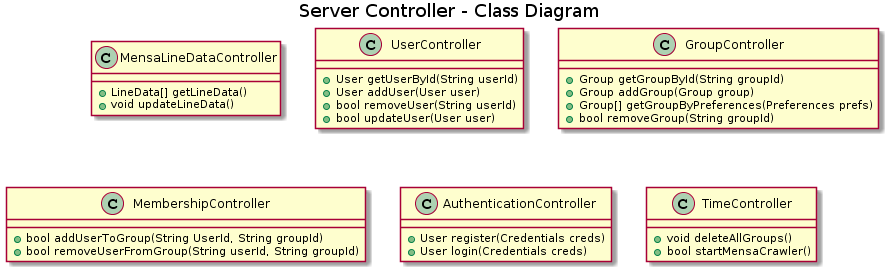
\includegraphics[width=1.1\textwidth]{Klassendiagramme/serverControllerCD.png}
\end{center}
\subsubsection{Class UserController}
\subsubsection*{Beschreibung}
Diese Klasse ist der User Controller und beinhaltet die für den User zuständigen Methoden

\subsubsection*{Methoden}
\begin{addmargin}[25pt]{0pt}
\begin{itemize}

\item \texttt{public User getUser(String userToken)}\\
	Mit dieser Methode wird eine Anfrage nach einem Userprofil gestellt. Es wird nach dem eindeutigen User Token gesucht
	\subsubsection*{Parameter}
	\begin{itemize}
	\item userToken \\
		Eindeutiger Token eines Userprofils
	\end{itemize}
	\subsubsection*{Rückgabewert}
	\begin{itemize}
	\item Userprofil
	\end{itemize}

\item \texttt{public User addUser(User user)}\\
	Diese Methode fügt einen User zur Datenbank hinzu
	\subsubsection*{Parameter}
	\begin{itemize}
	\item user \\
		Eindeutiges Userprofil
	\end{itemize}
	\subsubsection*{Rückgabewert}
	\begin{itemize}
	\item Userprofil
	\end{itemize}
	
\item \texttt{public bool removeUser(String userToken)}\\
	Diese Methode löscht ein Userprofil aus der Datenbank
	\subsubsection*{Parameter}
	\begin{itemize}
	\item userToken \\
		Eindeutiger Token eines Userprofils
	\end{itemize}
	\subsubsection*{Rückgabewert}
	\begin{itemize}
	\item Wird das Userprofil erfolgreich gelöscht, so wird eine Bestätigung zurückgegeben. Wenn der Löschvorgang fehlschlägt wird eine Fehlermeldung zurückgegeben
	\end{itemize}


\item \texttt{public bool updateUser(User user)}\\
	Diese Methode überschreibt ein bestehendes Userprofil mit einem Userprofil des selben Tokens, aber geänderten Parametern
	\subsubsection*{Parameter}
	\begin{itemize}
	\item user \\
		Eindeutiges Userprofil mit geänderten Parametern (bis auf Token)
	\end{itemize}
	\subsubsection*{Rückgabewert}
	\begin{itemize}
	\item Wird das Userprofil erfolgreich überschrieben, so wird eine Bestätigung zurückgegeben. Wenn das Überschreiben fehlschlägt wird eine Fehlermeldung zurückgegeben
	\end{itemize}
\end{itemize}

\end{addmargin}

\subsubsection{Class GroupController}
\subsubsection*{Beschreibung}
Diese Klasse ist der Group Controller und beinhaltet die für die Gruppen zuständigen Methoden

\subsubsection*{Methoden}
\begin{addmargin}[25pt]{0pt}
\begin{itemize}

\item \texttt{public Group getGroup(String groupToken)}\\
	Mit dieser Methode wird eine Anfrage nach einer Gruppe gestellt. Es wird nach dem eindeutigen Group Token gesucht
	\subsubsection*{Parameter}
	\begin{itemize}
	\item groupToken \\
		Eindeutiger Gruppen Token
	\end{itemize}
	\subsubsection*{Rückgabewert}
	\begin{itemize}
	\item Gruppe 
	\end{itemize}
	
\item \texttt{public Group addGroup(Group group)}\\
	Diese Methode fügt eine Gruppe zur Datenbank hinzu
	\subsubsection*{Parameter}
	\begin{itemize}
	\item group \\
		Gruppe mit korrekten Parametern
	\end{itemize}
	\subsubsection*{Rückgabewert}
	\begin{itemize}
	\item Die hinzugefügte Gruppe wird zurückgegeben
	\end{itemize}
	
\item \texttt{public Group[] getGroupByPreferences(Preferences prefs)}\\
	Diese Methode sucht nach Gruppen mit den passenden Präferenzen
	\subsubsection*{Parameter}
	\begin{itemize}
	\item prefs \\
		Nötige Präferenzen zur Findung einer passenden Gruppe (Linie und Uhrzeit)
	\end{itemize}
	\subsubsection*{Rückgabewert}
	\begin{itemize}
	\item Es werden alle Gruppen mit übereinstimmenden Präferenzen zurückgegeben
	\end{itemize}

\item \texttt{public bool removeGroup(String groupToken)}\\
	Diese Methode löscht eine Gruppe aus der Datenbank
	\subsubsection*{Parameter}
	\begin{itemize}
	\item groupToken \\
		Eindeutiger Group Token der zu löschenden Gruppe
	\end{itemize}
	\subsubsection*{Rückgabewert}
	\begin{itemize}
	\item Wird die Gruppe erfolgreich gelöscht, so wird eine Bestätigung zurückgegeben. Wenn der Löschvorgang fehlschlägt wird eine Fehlermeldung zurückgegeben
	\end{itemize}
\end{itemize}
\end{addmargin}

\subsubsection{Class MensaDataController}
\subsubsection*{Beschreibung}
Diese Klasse ist der Mensadaten Controller und enthält die Methoden, die für die Verwaltung der Mensadaten zuständig sind

\subsubsection*{Methoden}
\begin{addmargin}[25pt]{0pt}
\begin{itemize}

\item \texttt{public LineData[] getLineData()}\\
	Diese Methode fragt die Datenbank nach dem tagesaktuellen Speiseplan ab

	\subsubsection*{Rückgabewert}
	\begin{itemize}
	\item Es werden alle Essenslinien mit tagesaktuellem Menü zurückgegeben
	\end{itemize}
	
\item \texttt{public void updateLineData()}\\
	Diese Methode beinhaltet einen Crawler der den tagesaktuellen Speiseplan der Mensa vom Studentenwerk bezieht und anschließend in der Datenbank speichert
\end{itemize}
\end{addmargin}

\subsubsection{Class MembershipController}
\subsubsection*{Beschreibung}
Diese Klasse ist der Membership Controller und beinhaltet die Methoden, die für die Gruppenmitgliedschaft der einzelnen User zuständig sind

\subsubsection*{Methoden}
\begin{addmargin}[25pt]{0pt}
\begin{itemize}

\item \texttt{public bool addUserToGroup(String UserToken, String groupToken)}\\
	Diese Methode fügt einen User zu einer Gruppe hinzu
	\subsubsection*{Parameter}
	\begin{itemize}
	\item userToken \\
		Eindeutiger Token des Users der zur Gruppe hinzugefügt werden soll
	\item groupToken \\
		Eindeutiger Token der Gruppe, zu der der User hinzugefügt werden soll
	\end{itemize}
	\subsubsection*{Rückgabewert}
	\begin{itemize}
	\item Falls das Hinzufügen zur Gruppe erfolgreich war, wird eine Bestätigung zurückgegeben. Eine Fehlermeldung falls nicht.
	\end{itemize}
	
\item \texttt{public bool removeUserFromGroup(String userToken, String groupToken)}\\
	Diese Methode entfernt einen User aus einer Gruppe
	\subsubsection*{Parameter}
	\begin{itemize}
	\item userToken \\
		Eindeutiger Token des Users, der aus der Gruppe entfernt werden soll
	\item groupToken \\
		Eindeutiger Token der Gruppe, aus der der User entfernt werden soll
	\end{itemize}
	\subsubsection*{Rückgabewert}
	\begin{itemize}
	\item Falls das Entfernen aus der Gruppe erfolgreich war, wird eine Bestätigung zurückgegeben. Eine Fehlermeldung falls nicht.
	\end{itemize}
\end{itemize}
\end{addmargin}

\subsubsection{Class AuthenticationController}
\subsubsection*{Beschreibung}
Diese Klasse ist der Authentication Controller und beinhaltet die Methoden, die für die Registrierung und das Anmelden eines Users zuständig sind

\subsubsection*{Methoden}
\begin{addmargin}[25pt]{0pt}
\begin{itemize}

\item \texttt{public User register(Credentials creds)}\\
	Diese Methode ist für die Registrierung eines Users zuständig
	\subsubsection*{Parameter}
	\begin{itemize}
	\item creds \\
		Die vom User festgelegten Daten zur Registrierung, bestehend aus E-Mail und Passwort
	\end{itemize}
	\subsubsection*{Rückgabewert}
	\begin{itemize}
	\item Es wird ein leeres Userprofil zurückgegeben
	\end{itemize}
	
\item \texttt{public User login(Credentials creds)}\\
	Diese Methode ist für die Ameldung eines Users zuständig
	\subsubsection*{Parameter}
	\begin{itemize}
	\item creds \\
		Die vom User bei der Registrierung festgelegten Daten, bestehend aus E-Mail und Passwort
	\end{itemize}
	\subsubsection*{Rückgabewert}
	\begin{itemize}
	\item Es wird das UserProfil des Users zurückgegeben
	\end{itemize}

\end{itemize}
\end{addmargin}

\subsubsection{Class TimeController}
\subsubsection*{Beschreibung}
Diese Klasse ist der Time Controller und beinhaltet die Methoden, die für die zeitlich festgelegte Abläufe zuständig ist

\subsubsection*{Methoden}
\begin{addmargin}[25pt]{0pt}
\begin{itemize}

\item \texttt{public void deleteAllGroups()}\\
	Diese Methode löscht am Ende des Tages alle Gruppen
	
\item \texttt{public bool startMensaCrawler()}\\
	Diese Methode startet jeden Morgen den Aufruf zum Abrufen der Mensadaten
	\subsubsection*{Rückgabewert}
	\begin{itemize}
	\item Wurden die Mensadaten erfolgreich abgegriffen, wird eine Bestätigung zurückgegeben. Eine Fehlermeldung falls nicht.
	\end{itemize}

\end{itemize}
\end{addmargin}

\newpage
\section{HTTP Protokoll}

Die REST Endpoints die in der Tabelle aufgelistet sind werden für die Kommunikation zwischen Client und Server verwendet. \\

\resizebox{16cm}{!} {
\begin{tabu} { | l | l | l | l | } 
 \hline
 Request Type & Endpoint & Payload & Beschreibung \\ [0.5ex] 
 \hline
 GET  & /user/\{token\} &  & Liefert den User mit dem übergebenem Token. \\ 
 
 POST & /user  & User & Updated den User (Token liegt in User) \\ 
 \hline
GET & /group/{token} & & Liefert die Gruppe mit dem übergebenem Token. \\
POST & /group-prefferences & Preferrences & Liefert alle Gruppen die zu den übergebenen Prefferenzen passen. \\
POST  & /create-group/  & Group & Erstellt die übergebene Gruppe. \\
DELETE  & /group/\{token\} & & Löscht die Gruppe mit dem übergebenen Token. \\

\hline 

POST  & /add-user-to-group?user=\{userToken\}\&group={groupToken} & & Fügt den User mit dem userToken zu der Gruppe mit dem groupToken. \\
POST  & /remove-user-from-group?user=\{userToken\}\&group={groupToken} & & Entfernt den User mit dem userToken von der Gruppe mit dem groupToken. \\

\hline

POST & /login & email, password & Meldet den Client an dem Account mit den übergebenen Anmeldedaten an. \\
POST & /register & email, password & Erstellt einen Account mit den übergebenen Anmeldedaten. \\

\hline

GET &  /mensadata & & Liefert die aktuellen Mensadaten.\\

\hline

\end{tabu}
}




\chapter{Datenstrukturen}

\begin{center}
	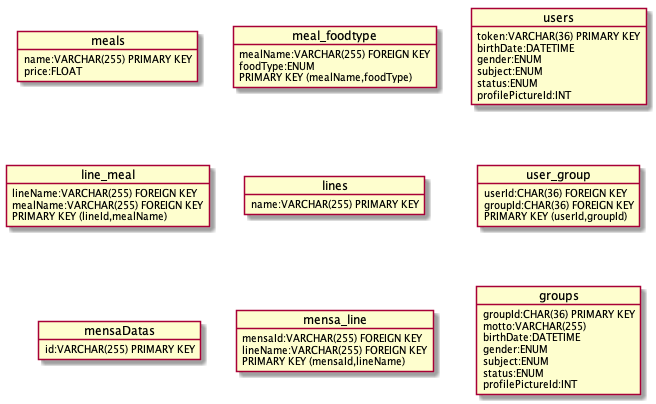
\includegraphics[width=0.93\textwidth]{Objektdiagramme/datenstrukturen.png}
\end{center}
In der Abbildung sieht man die Datenstruktur der Datenbank, also die Tabellen, die es in der Datenbank geben wird. Weil wir mySQL verwenden und mySQL nicht List-Type als Datentype unterstützt, speichern wir Liste in Form von extra Tabellen.

\chapter{Dynamische Modelle}

\section{Sequenzdiagramme}
Es werden nun einige Abläufe innerhalb der App  MensaMeet durch Sequenzdiagramme veranschaulicht. 
\subsection{Registrieren}
\begin{center}
	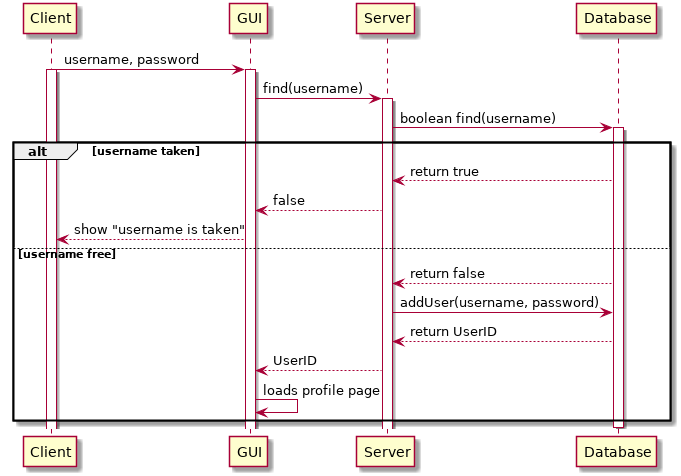
\includegraphics[width=0.93\textwidth]{Sequenzdiagramme/Registration.png}
\end{center}
\subsection*{Beschreibung}
Bob öffnet zum ersten mal die \GLS{Applikation} MensaMeet und sieht den Registrierungsbildschrim. Dort soll er seine E-Mailadresse und ein Passwort eingeben. Sobald er das getan hat, werden die Daten an der Server geschickt, welcher sie an Firebase weiterleitet. Firebase legt auf seinem Server den User an und generiert ein Token zur UserIdentifikation. Das Token wird an den Server zurückgegeben, der damit einen User in der Datenbank anlegt und das Userobjekt an den Client schickt. Auf dem Client (Bobs Smartphone) wird der User/Token gespeichert und bei jeder zukünftigen Anfrage an den Server mitgegeben. 
Bob sieht nun den Bildschirm zur Profilbearbeitung. Die Eingabe der Profildaten ist Pflicht, vorher kann er nicht weiter zu einer anderen Seite gelangen.
Nachdem er seinen Nutzernamen, Motto, Alter, Geschlecht, Status, Fachrichtung eingegeben hat, werden diese Daten an den Server gesendet, der damit das Userprofil in der Datenbank aktualisiert. 
\newpage
\subsection{Mensalinien wählen}
\begin{center}
	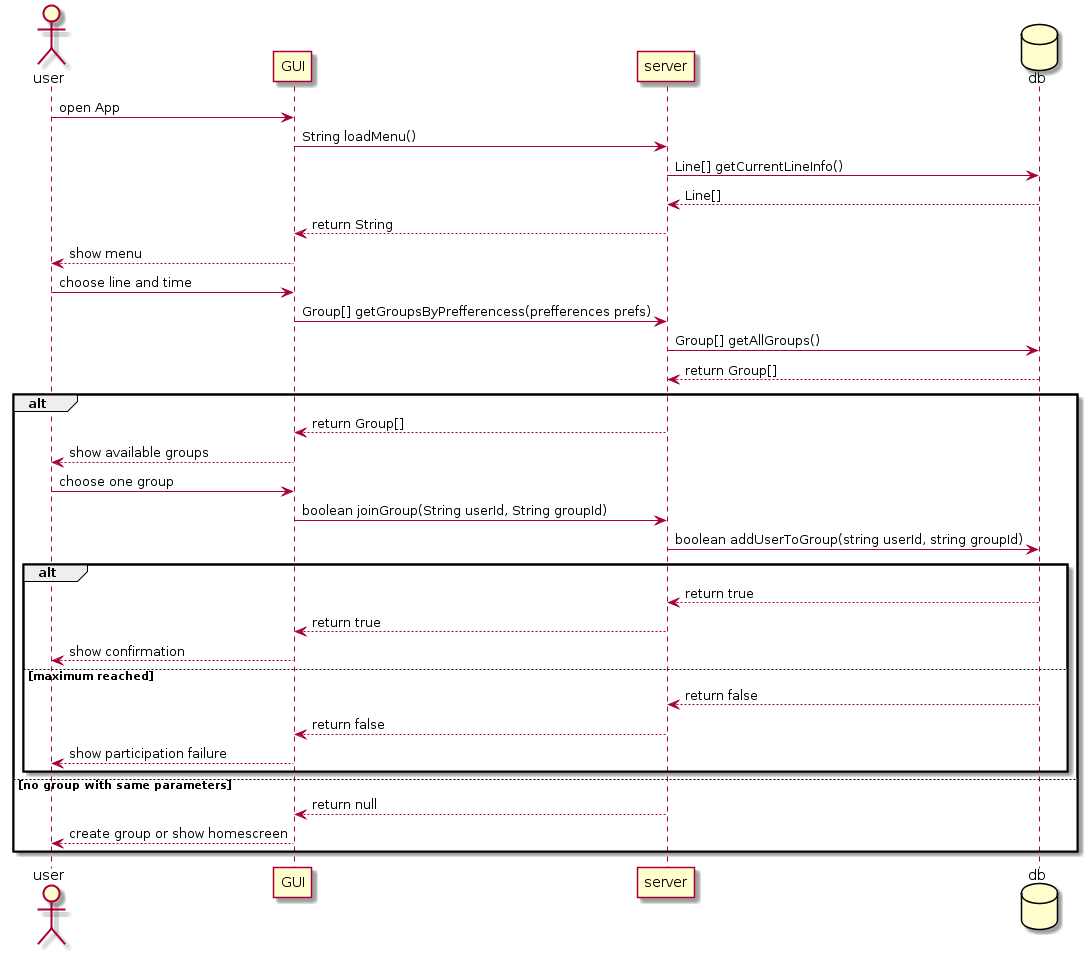
\includegraphics[width=0.93\textwidth]{Sequenzdiagramme/chooseLineAndTimeSD.png}
\end{center}
\subsection*{Beschreibung}
Der Nutzer öffnet die Anwendung (die Registrierung ist bereits erfolgt). Nun soll er als Scrolldown-menü die Mensalinien mit ihrem jeweiligen Angebot zu sehen kriegen (Dies ist der "HomeScreen"). Dazu werden die Mensadaten über den Server von der Datenbank angefragt, aufbereitet und dem Client übermittelt. Dieser kann nun die Linien anklicken an denen er gern essen möchte. Danach stellt er das für ihn geeignete Zeitintervall ein. Diese Daten werden dem Server übermittelt, welcher sich die Gruppen aus der Datenbank holt, nach den angegebenen Daten filtert und an den Client übergibt. Der Nutzer kann sich die Gruppen anschauen und einer davon beitreten. Beim Versuch beizutreten wird dem Server der User- und der GroupToken übermittelt. Es wird überprüft ob die Gruppe bereits voll ist, ist dies der Fall, erhält der Client eine Fehlermeldung und gelangt wieder zur Gruppenübersicht. Ist noch Platz in der Gruppe, wird die Gruppe in der Datenbank aktualisiert, indem der User hinzugefügt wird. Dann wird über den Server eine Bestätigung an den Client geschickt und der Nutzer gelangt zur Gruppenseite. 
Falls keine Gruppen passend zu den Angaben des Clients gefunden wurde, erhält der Client eine passende Fehlermeldung und kann entweder zurück zum HomeScreen oder selbst eine Gruppe erstellen.

\newpage
\subsection{Gruppe beitreten}
\begin{center}
	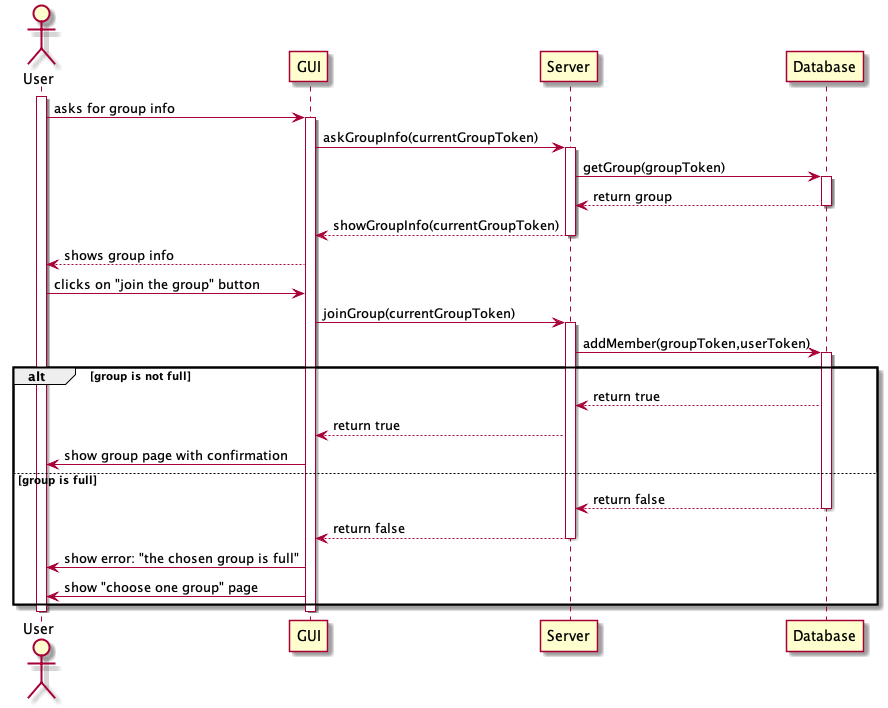
\includegraphics[width=0.93\textwidth]{Sequenzdiagramme/checkInfoAndJoinGroupSD.png}
\end{center}


\subsection*{Beschreibung}
Nachdem der Nutzer, passend zu seinen ausgewählten Linien und seinem eingestellten Zeitintervall, Gruppen in einem Scrolldown-menü angezeigt bekam, klickt er nun eine Gruppe an, um mehr Informationen zu ihr zu sehen. Dazu wird an den Server eine Anfrage mit dem GroupToken gesendet. Der Server sucht damit nach der Gruppe in der Datenbank und übermittelt die Informationen dem Client. Beim User wird die angeklickte Gruppe nach unten aufgklappt, so dass nun zusätzlich zur Linie, Startzeit und Motto auch die Mitgliederliste und den "Beitreten"-Button sieht. Er drückt auf "Beitreten". Nun wird dem Server die UserID und GroupID übermittelt. Er prüft in der Datenbank ob die Gruppe inzwischen voll ist. Ist dies der Fall, erhält der Client eine Fehlermeldung : "Deine gewählte Gruppe ist bereits voll" und gelangt wieder zur Gruppenübersicht. Ist noch Platz in der Gruppe, wird die Datenbank aktualisiert und dem Client der Beitritt bestätigt. Der Nutzer gelangt zur Detailansicht seiner Gruppe. Er steht nun ebenfalls in der Mitgliederliste und sieht den Button "Gruppe Verlassen".

\newpage
\subsection{Gruppe erstellen}
\begin{center}
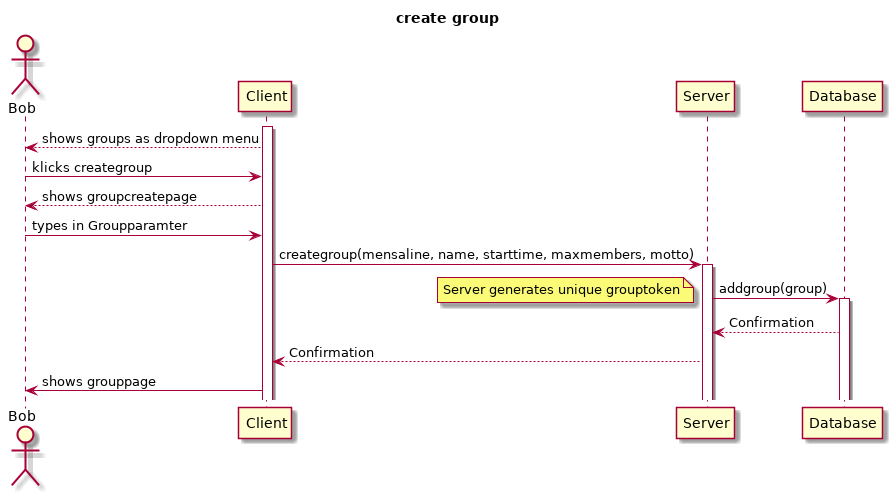
\includegraphics[width=0.93\textwidth]{Sequenzdiagramme/CreateGroup.png}

\end{center}
\subsection*{Beschreibung}
Nachdem der User die zu ihm passenden Gruppen angefragt hat, aber keine gefunden wurde entscheidet er sich eine Gruppe zu erstellen. Er stellt dazu die erforderlichen Gruppenparameter(Gruppenname, Mensalinie, Startzeit, Motto, Maximale Mitgliederzahl) ein. Der Server erhält die Anfrage mit diesen Paramtern eine neue Gruppe anzulegen. Er generiert (aus dem Namen?) ein eindeutiges groupToken und legt die Gruppe in der Datenbank an. Dem Client wird die erfolgreiche Gruppengründung bestätigt und ihm wird als nächstes die Detailansicht seiner Gruppe angezeigt.

\newpage
\subsection{Gruppe verlassen}
\begin{center}
	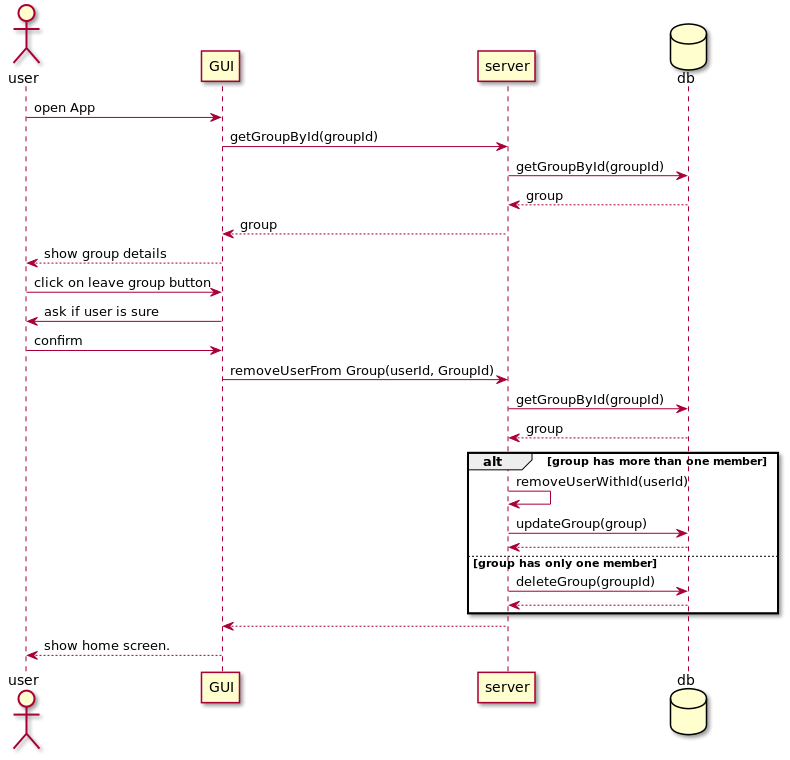
\includegraphics[width=0.93\textwidth]{Sequenzdiagramme/leaveGroupSD.png}
\end{center}

\subsection*{Beschreiung}
Der Nutzer öffnet die App MensaMeet. Da er bereits Mitglied einer Gruppe ist, wird ihm die Detailansicht seiner Gruppe angezeigt.
In dieser Ansicht ist ein Button "Gruppe verlassen". Er drückt diesen Button und muss seine Entscheidung bestätigen. Für den Austritt wird dem Server der User- und GroupToken übermittelt. Der Server sucht anhand des GroupToken die Gruppe in der Datenbank um sie zu aktualisieren. Der User wird aus der Gruppe entfernt und die Mitgliederzahl der Gruppe überprüft. Ist diese nun bei 0, so wird die Gruppe aus der Datenbank gelöscht.
Der Client erhält in jedem Fall die Bestätigung zum Austritt aus der Gruppe und wird wieder zum HomeScreen überführt.


\chapter{Änderungen zum Pflichtenheft}
\begin{itemize}
	\item Nutzername und Gruppennamen müssen nicht mehr eindeutig sein \\
	stattdessen wird für den Nutzer von Firebase ein eindeutiges Token generiert, das als Identifikator dient. Für Gruppen wird ebenfalls ein eindeutiges Token durch den Server generiert.
	\item Zum Registrieren wird statt Nutzername und Password nun Email und Passwort benötigt. \\Diese Änderung ist bedingt durch die Nutzung von Firebase und erfüllt damit eines unserer Wunschkriterien: Dass eine Email Verifikation beim Registrieren stattfindet. 
\end{itemize}

\printglossaries

\chapter{Anhang}
\section{Klassendiagramm Client-Server}
\begin{center}
	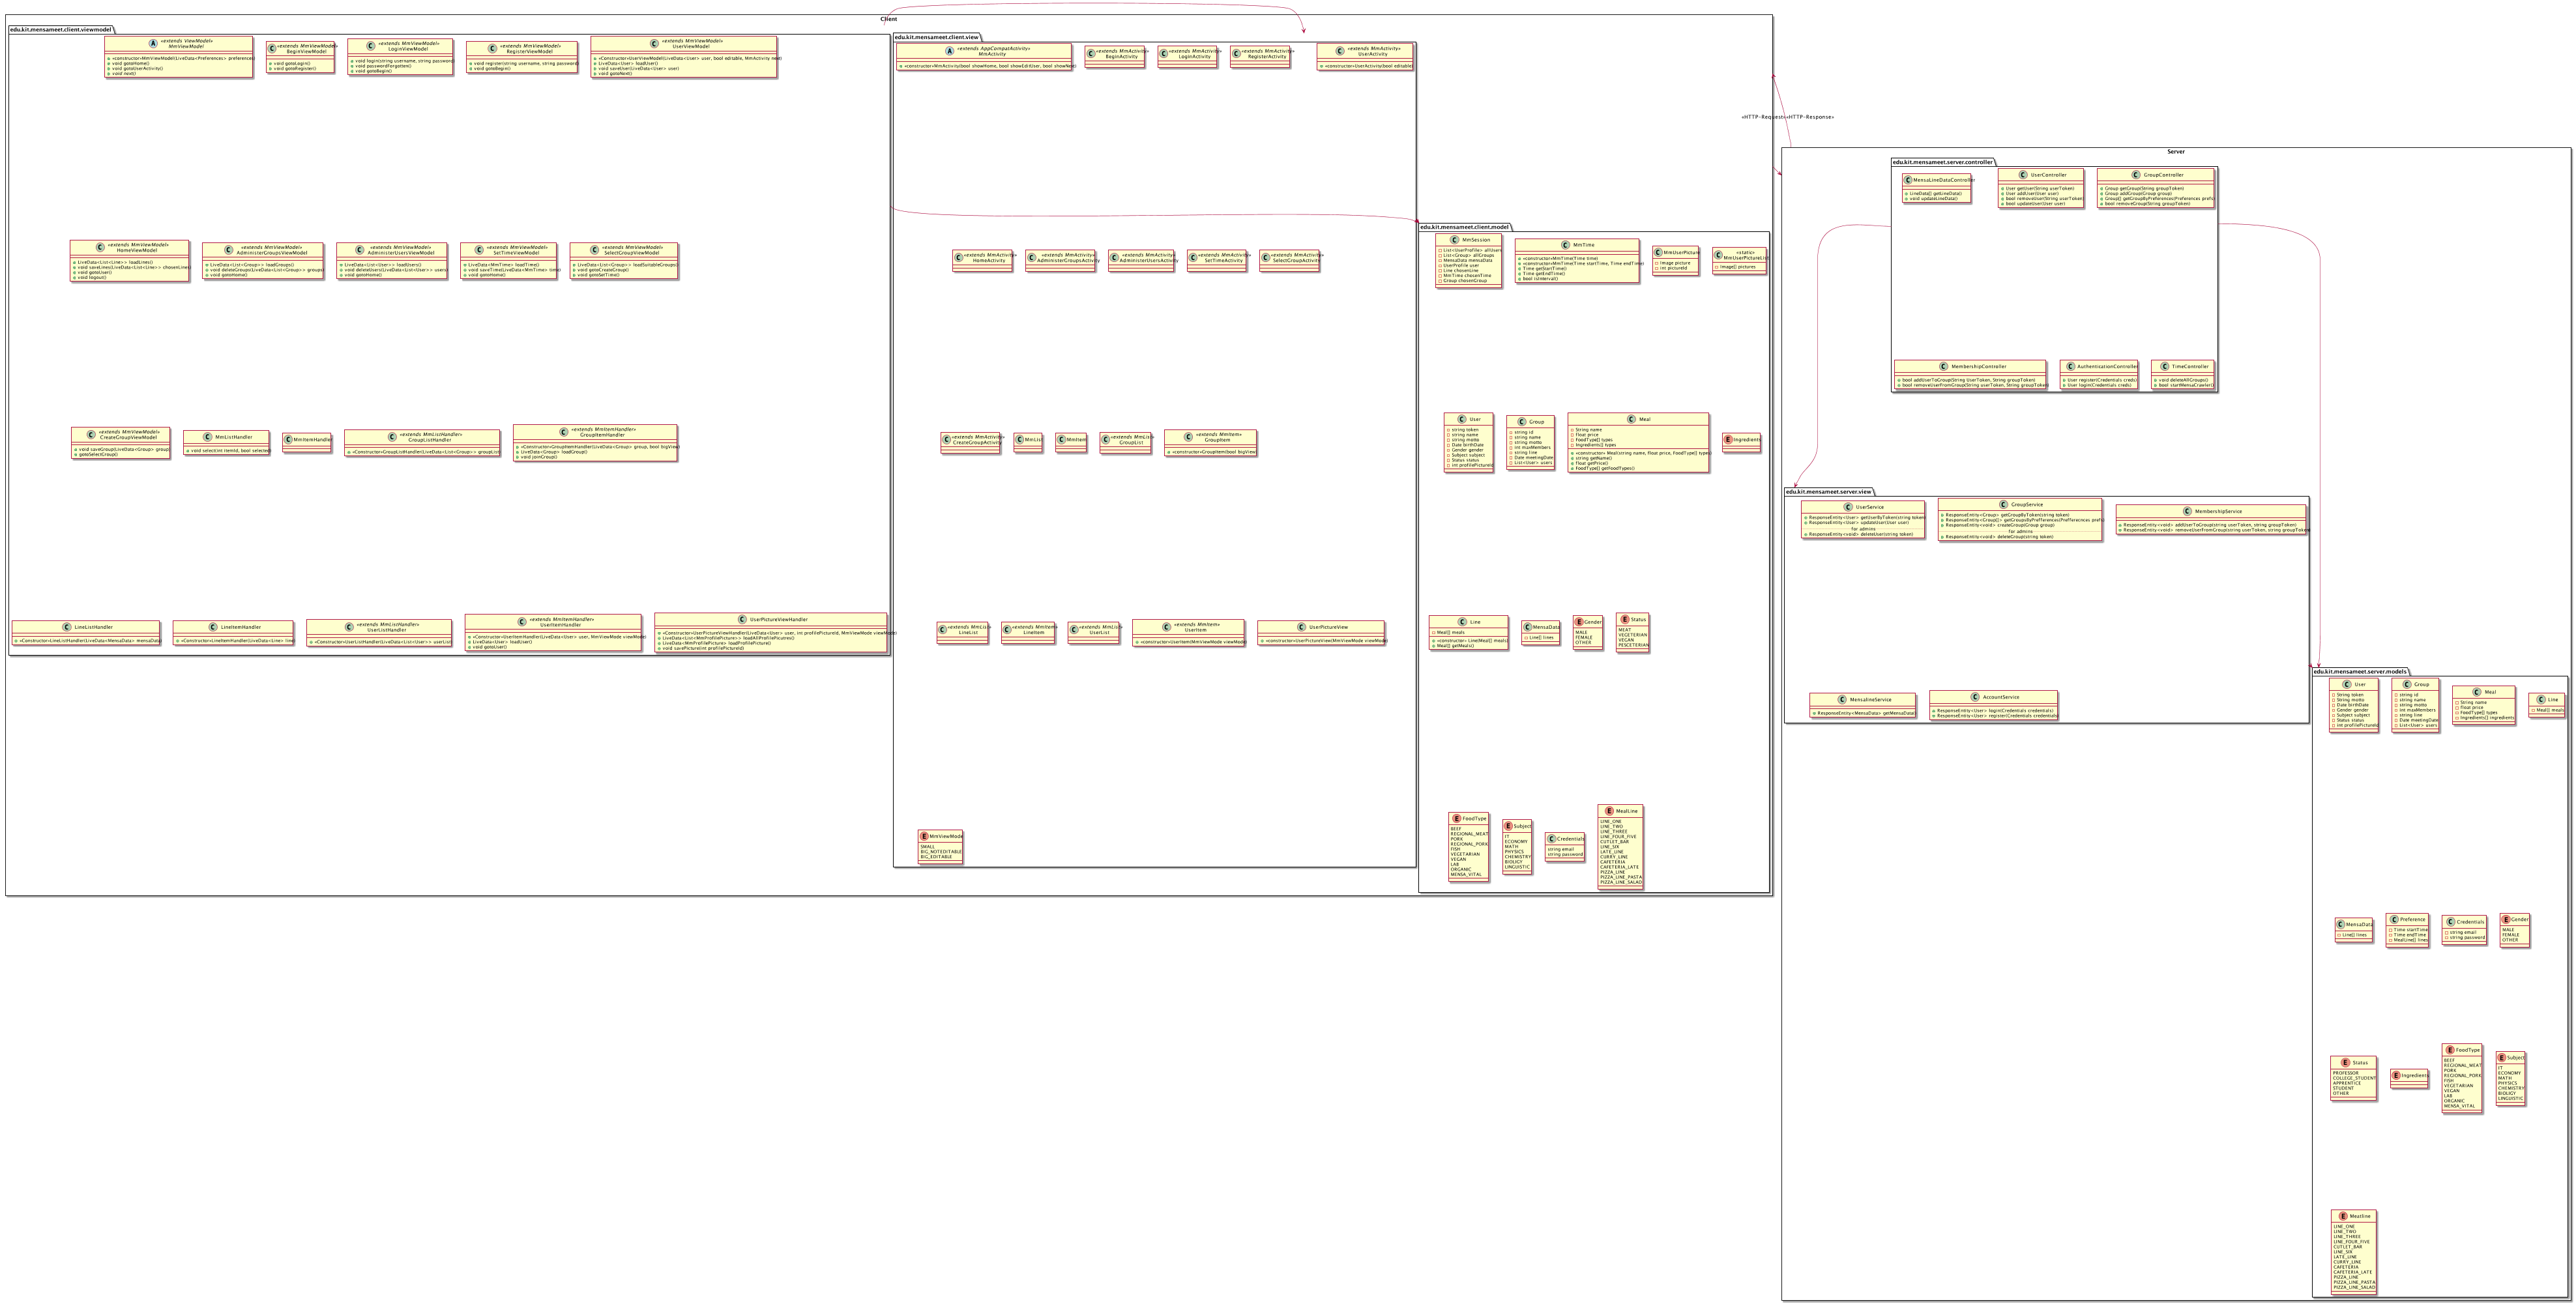
\includegraphics[width=0.93\textwidth]{Klassendiagramme/client_server.png}
\end{center}

\end{document}
